%! TEX root = **/010-main.tex
% vim: spell spelllang=en:

%%%%%%%%%%%%%%%%%%%%%%%%%%%%%%%%%%%%%%%%%%%%%%%%%%%%%%%%%%%%%%%%%%%%%%%%%%%%%%%%
% PREAMBLE
%%%%%%%%%%%%%%%%%%%%%%%%%%%%%%%%%%%%%%%%%%%%%%%%%%%%%%%%%%%%%%%%%%%%%%%%%%%%%%%%
%! TEX root = **/010-main.tex
%%%%%%%%%%%%%%%%%%%%%%%%%%%%%%%%%%%%%%%%%%%%%%%%%%%%%%%%%%%%%%%%%%%%%%%%%%%%%%%%
%% LaTeX preamble, load in main.tex with: \input{preamble}
%%%%%%%%%%%%%%%%%%%%%%%%%%%%%%%%%%%%%%%%%%%%%%%%%%%%%%%%%%%%%%%%%%%%%%%%%%%%%%%%

\documentclass[12pt, oneside, final]{article}
% \usepackage[a4paper, left=2.5cm, right=2.5cm, top=2.5cm, bottom=2.5cm]{geometry}
\usepackage[a4paper]{geometry}
% \usepackage[a4paper,showframe]{geometry}

\setlength{\headheight}{24pt}

% for debugging overfulls
%\documentclass[draft, 12pt, oneside]{article}
%\usepackage[showframe, a4paper, left=2.5cm, right=2.5cm, top=2.5cm, bottom=2.5cm]{geometry}

%%%%%%%%%%%%%%%%%%%%%%%%%%%%%%%%%%%%%%%%%%%%%%%%%%%%%%%%%%%%%%%%%%%%%%%%%%%%%%%%
%% FONTS
%%%%%%%%%%%%%%%%%%%%%%%%%%%%%%%%%%%%%%%%%%%%%%%%%%%%%%%%%%%%%%%%%%%%%%%%%%%%%%%%

\usepackage[T1]{fontenc}
\usepackage{fontspec}
\usepackage{microtype}

\setmonofont[Scale=MatchLowercase]{DejaVu Sans Mono}

%%%%%%%%%%%%%%%%%%%%%%%%%%%%%%%%%%%%%%%%%%%%%%%%%%%%%%%%%%%%%%%%%%%%%%%%%%%%%%%%
%% LANGUAGE
%%%%%%%%%%%%%%%%%%%%%%%%%%%%%%%%%%%%%%%%%%%%%%%%%%%%%%%%%%%%%%%%%%%%%%%%%%%%%%%%

\usepackage{polyglossia}
\setdefaultlanguage{english}
\setotherlanguages{spanish,catalan}

%%%%%%%%%%%%%%%%%%%%%%%%%%%%%%%%%%%%%%%%%%%%%%%%%%%%%%%%%%%%%%%%%%%%%%%%%%%%%%%%
%% BIBLIOGRAPHY
%%%%%%%%%%%%%%%%%%%%%%%%%%%%%%%%%%%%%%%%%%%%%%%%%%%%%%%%%%%%%%%%%%%%%%%%%%%%%%%%

\usepackage[
    backend=biber,
    style=numeric,
]{biblatex}
\DeclareNameAlias{default}{family-given}

\addbibresource{biblio.bib}

\usepackage{fvextra}        % Req by minted (must load before csquotes)
\usepackage{csquotes}       % For bibliography quotations
\DeclareQuoteAlias{spanish}{catalan}

%%%%%%%%%%%%%%%%%%%%%%%%%%%%%%%%%%%%%%%%%%%%%%%%%%%%%%%%%%%%%%%%%%%%%%%%%%%%%%%%
%% COMMON
%%%%%%%%%%%%%%%%%%%%%%%%%%%%%%%%%%%%%%%%%%%%%%%%%%%%%%%%%%%%%%%%%%%%%%%%%%%%%%%%

\usepackage{color, xcolor}     % more colors

\usepackage{graphicx}   % graphics
\graphicspath{{./figures/}}

\usepackage{comment}

%%%%%%%%%%%%%%%%%%%%%%%%%%%%%%%%%%%%%%%%%%%%%%%%%%%%%%%%%%%%%%%%%%%%%%%%%%%%%%%%
%% MATHS
%%%%%%%%%%%%%%%%%%%%%%%%%%%%%%%%%%%%%%%%%%%%%%%%%%%%%%%%%%%%%%%%%%%%%%%%%%%%%%%%

\usepackage{mathtools}  % amsmath + more
\usepackage{amsthm}     % Theorem enviroment
\usepackage{amssymb}    % More symbols
\usepackage{amstext}    % Text inside mathenv

%\usepackage{relsize}    % Bigger math with mathlarger{___}
\usepackage{nicefrac}   % nice fractions in one line

%\usepackage{IEEEtrantools} % Complex equation arrays

%%%%%%%%%%%%%%%%%%%%%%%%%%%%%%%%%%%%%%%%%%%%%%%%%%%%%%%%%%%%%%%%%%%%%%%%%%%%%%%%
%% REFERENCES (load order is important)
%%%%%%%%%%%%%%%%%%%%%%%%%%%%%%%%%%%%%%%%%%%%%%%%%%%%%%%%%%%%%%%%%%%%%%%%%%%%%%%%

\usepackage{varioref} % reference far away (1)
\usepackage[colorlinks = true]{hyperref} % links in references (2)
\usepackage{cleveref} % smart references (3)
%hyperref configuration so that it doesn't contrast so much colorlinks,
\hypersetup{
   linkcolor={black},
   citecolor={black},
   %linkcolor={red!50!black},
   %citecolor={blue!50!black},
   urlcolor={blue!80!black}
}

\usepackage[bottom]{footmisc} % Footnotes at bottom of page

%%%%%%%%%%%%%%%%%%%%%%%%%%%%%%%%%%%%%%%%%%%%%%%%%%%%%%%%%%%%%%%%%%%%%%%%%%%%%%%%
%% FIGURES
%%%%%%%%%%%%%%%%%%%%%%%%%%%%%%%%%%%%%%%%%%%%%%%%%%%%%%%%%%%%%%%%%%%%%%%%%%%%%%%%

%\usepackage[export]{adjustbox}  % Adjust table size
\usepackage{float}               % Force tables and images position (H and H!)
%\usepackage{wrapfig}            % Wrap images like in HTML

\usepackage[justification=centering]{caption}
%\usepackage{subcaption}                     % Subfigures
%\usepackage[framemethod=tikz]{mdframed}     % Custom frames

%%%%%%%%%%%%%%%%%%%%%%%%%%%%%%%%%%%%%%%%%%%%%%%%%%%%%%%%%%%%%%%%%%%%%%%%%%%%%%%%
%% TABLES
%%%%%%%%%%%%%%%%%%%%%%%%%%%%%%%%%%%%%%%%%%%%%%%%%%%%%%%%%%%%%%%%%%%%%%%%%%%%%%%%

%\usepackage{colortbl, booktabs} % Better tables
%\usepackage{tabularx}
%\usepackage{longtable} % Multiple page table (does not work with tabularx)
\usepackage{xltabular, colortbl, booktabs} % longtable + tabularx (has bug with booktabs: fix below)

% Split cell in lines and more formating options inside table
\usepackage{array, multirow, multicol, makecell}

%%%
% bug fix for booktabs + xltabular incompatibility
\makeatletter
\def\@BTrule[#1]{%
  \ifx\longtable\undefined
    \let\@BTswitch\@BTnormal
  \else\ifx\hline\LT@hline
    \nobreak
    \let\@BTswitch\@BLTrule
  \else
     \let\@BTswitch\@BTnormal
  \fi\fi
  \global\@thisrulewidth=#1\relax
  \ifnum\@thisruleclass=\tw@\vskip\@aboverulesep\else
  \ifnum\@lastruleclass=\z@\vskip\@aboverulesep\else
  \ifnum\@lastruleclass=\@ne\vskip\doublerulesep\fi\fi\fi
  \@BTswitch}
\makeatother
%%%

%%%%%%%%%%%%%%%%%%%%%%%%%%%%%%%%%%%%%%%%%%%%%%%%%%%%%%%%%%%%%%%%%%%%%%%%%%%%%%%%
%% SIUNITX
%%%%%%%%%%%%%%%%%%%%%%%%%%%%%%%%%%%%%%%%%%%%%%%%%%%%%%%%%%%%%%%%%%%%%%%%%%%%%%%%

\usepackage{siunitx}                        % SI units and uncertainties
%\sisetup{locale = FR}                       % Commas and so on for spanish
%\sisetup{separate-uncertainty=true}
\sisetup{
  per-mode=fraction,
  fraction-function=\nicefrac
}

%%%%%%%%%%%%%%%%%%%%%%%%%%%%%%%%%%%%%%%%%%%%%%%%%%%%%%%%%%%%%%%%%%%%%%%%%%%%%%%%
%% TIKZ
%%%%%%%%%%%%%%%%%%%%%%%%%%%%%%%%%%%%%%%%%%%%%%%%%%%%%%%%%%%%%%%%%%%%%%%%%%%%%%%%

%\usepackage{tikz}
%\usetikzlibrary{arrows}
%\usetikzlibrary{scopes}
%\usetikzlibrary{babel}

%%%%%%%%%%%%%%%%%%%%%%%%%%%%%%%%%%%%%%%%%%%%%%%%%%%%%%%%%%%%%%%%%%%%%%%%%%%%%%%%
%% MINTED
%%%%%%%%%%%%%%%%%%%%%%%%%%%%%%%%%%%%%%%%%%%%%%%%%%%%%%%%%%%%%%%%%%%%%%%%%%%%%%%%

\usepackage{minted}
\definecolor{codeBg}{HTML}{FFFDE7}
\setminted{
    %style=pastie,
    frame=lines,
    framesep=3mm,
    linenos,
    breaklines=true,
    encoding=utf8,
    fontsize=\footnotesize,
    bgcolor=codeBg
}

%%%%%%%%%%%%%%%%%%%%%%%%%%%%%%%%%%%%%%%%%%%%%%%%%%%%%%%%%%%%%%%%%%%%%%%%%%%%%%%%
%% CUSTOM COMMANDS
%%%%%%%%%%%%%%%%%%%%%%%%%%%%%%%%%%%%%%%%%%%%%%%%%%%%%%%%%%%%%%%%%%%%%%%%%%%%%%%%

% empty whitepage without numbering
\newcommand{\whitepage}{
    \clearpage\thispagestyle{empty}\addtocounter{page}{-1} \newpage \clearpage
}

% Add command before appendix section for page numbering: A-1
\newcommand{\appendixpagenumbering}{
    \break
    \pagenumbering{arabic}
    \renewcommand{\thepage}{\thesection-\arabic{page}}
}

%%%%%%%%%%%%%%%%%%%%%%%%%%%%%%%%%%%%%%%%%%%%%%%%%%%%%%%%%%%%%%%%%%%%%%%%%%%%%%%%
%% CUSTOM MATH OPERATORS (functions not in italic in math mode)
%%%%%%%%%%%%%%%%%%%%%%%%%%%%%%%%%%%%%%%%%%%%%%%%%%%%%%%%%%%%%%%%%%%%%%%%%%%%%%%%

%\DeclareMathOperator{\arcsec}{arcsec}
%\DeclareMathOperator{\arccot}{arccot}
%\DeclareMathOperator{\arccsc}{arccsc}
%\DeclareMathOperator{\cis}{cis}

%%%%%%%%%%%%%%%%%%%%%%%%%%%%%%%%%%%%%%%%%%%%%%%%%%%%%%%%%%%%%%%%%%%%%%%%%%%%%%%%
%% MISC
%%%%%%%%%%%%%%%%%%%%%%%%%%%%%%%%%%%%%%%%%%%%%%%%%%%%%%%%%%%%%%%%%%%%%%%%%%%%%%%%

%\usepackage{datetime} % Customize date
%% \monthyeardate\today gives the date without the day
%\newdateformat{monthyeardate}{%
    %\monthname[\THEMONTH], \THEYEAR}


%%%%%%%%%%%%%%%%%%%%%%%%%%%%%%%%%%%%%%%%%%%%%%%%%%%%%%%%%%%%%%%%%%%%%%%%%%%%%%%%
% EXTRA PACKAGES / CONFIG
%%%%%%%%%%%%%%%%%%%%%%%%%%%%%%%%%%%%%%%%%%%%%%%%%%%%%%%%%%%%%%%%%%%%%%%%%%%%%%%%

% \includeonly{
%     060-convergence-analysis,
%     070-initial-cuda
% }

\usepackage{fancyhdr}
\usepackage{pgfgantt}
\usepackage{pdflscape}
\usepackage{titlesec}

\usepackage{chngcntr}
\counterwithin{figure}{section}
\counterwithin{table}{section}

% paragraph in newline
\titleformat{\paragraph}[hang]{\normalfont\normalsize\bfseries}{\theparagraph}{1em}{}
\titlespacing*{\paragraph}{0pt}{3.25ex plus 1ex minus .2ex}{0.5em}

% bold \thead (table headers)
\renewcommand\theadfont{\bfseries}

%%%%%%%%%%%%%%%%%%%%%%%%%%%%%%%%%%%%%%%%%%%%%%%%%%%%%%%%%%%%%%%%%%%%%%%%%%%%%%%%
% METADATA
%%%%%%%%%%%%%%%%%%%%%%%%%%%%%%%%%%%%%%%%%%%%%%%%%%%%%%%%%%%%%%%%%%%%%%%%%%%%%%%%
\title{High-performance simulation of the 16th Hilbert's problem}
\author{Aleix Bon\'e Rib\'o}
\date{\today}

\begin{document}
%%%%%%%%%%%%%%%%%%%%%%%%%%%%%%%%%%%%%%%%%%%%%%%%%%%%%%%%%%%%%%%%%%%%%%%%%%%%%%%%
% TITLE
%%%%%%%%%%%%%%%%%%%%%%%%%%%%%%%%%%%%%%%%%%%%%%%%%%%%%%%%%%%%%%%%%%%%%%%%%%%%%%%%

    % Default title or use titlepage.tex

    %\maketitle
    %! TEX root = **/010-main.tex
% vim: spell spelllang=en:

\thispagestyle{empty}
\clearpage
\setcounter{page}{-1}

\makeatletter
\begin{titlepage}
{
    \centering
    
\includegraphics[width=0.9\textwidth]{logo-upc}
    \null
    \vspace{3em}
    {\Huge \bfseries \@title \par}
    \vspace{2em}
    {\large Project management (GEP) \\
        (Budget and sustainability) %todo change
    \par}
    \vspace{3em}
    {\large \scshape \@date \par}

    \vfill
    {\raggedleft \large \bfseries \@author \par}
    \vspace{1em}
    {\raggedleft \large
        Bachelor thesis \\
        Specialization in Computing \\
        \vspace{2em}
        Director: Grigori Astrakharchik \\
        GEP Tutor: Eguiguren Huerta Marcos
    \par}
}
\end{titlepage}
\makeatother


%%%%%%%%%%%%%%%%%%%%%%%%%%%%%%%%%%%%%%%%%%%%%%%%%%%%%%%%%%%%%%%%%%%%%%%%%%%%%%%%
% TOC & lists
%%%%%%%%%%%%%%%%%%%%%%%%%%%%%%%%%%%%%%%%%%%%%%%%%%%%%%%%%%%%%%%%%%%%%%%%%%%%%%%%

    \pagenumbering{Roman}

    %\setcounter{tocdepth}{2}
    \tableofcontents \pagebreak

    \listoffigures \pagebreak
    \listoftables
    \listoflistings
    \clearpage

    \pagenumbering{arabic}

%%%%%%%%%%%%%%%%%%%%%%%%%%%%%%%%%%%%%%%%%%%%%%%%%%%%%%%%%%%%%%%%%%%%%%%%%%%%%%%%
% SECTIONS
%%%%%%%%%%%%%%%%%%%%%%%%%%%%%%%%%%%%%%%%%%%%%%%%%%%%%%%%%%%%%%%%%%%%%%%%%%%%%%%%

    % Paragraph spacing (placed after ToC)
    \setlength{\parskip}{1em plus 0.5em minus 0.2em}
    %\setlength{\parindent}{0pt}

\null\vfill
\vspace{-5em}
\begin{abstract}
    A high performance program to find limit cycles in quadratic ordinary systems of
    equations (ODEs) using the computational power of GPUs (Graphical Processing Units)
    was developed. The program is able to find limit cycles on a quadratic system
    in seconds, allowing for a quick visualization of the cycles or to perform a massive
    parameter search to find systems with interesting limit cycle configurations.
\end{abstract}
\vfill\null
\pagebreak

    \pagestyle{fancy}
    \fancyhf{}


    \makeatletter
        \fancyhead[L]{\@title}
        \fancyfoot[L]{Chapter \thesection}
        \fancyfoot[C]{\@author}
        \fancyfoot[R]{\thepage}
    \makeatother

    \renewcommand{\headrulewidth}{1pt}
    \renewcommand{\footrulewidth}{0.75pt}

    % GEP
    %! TEX root = **/010-main.tex
% vim: spell spelllang=en:

\section{Context and scope}%
\label{sec:context}

\subsection{Introduction and contextualization}%
\label{sub:intro}

Since its release in 2007, Compute Unified Device Architecture (CUDA) has
revolutionized the usage of graphic processing units for scientific
computations, allowing developers to implement programs that take full advantage
of the parallelization capabilities of GPUs for general purpose programming.
This paired with the exponential growth of computing power that GPUs have
experienced in the last decade has made GPU numerical analysis essential on
modern science research. Highly complex problems that where once impossible to
compute in realistic time frames can now be computed even on average consumer
hardware GPUs. Moreover, projects like
\emph{GPUGRID}\footnote{\url{www.gpugrid.net}} allow researches to run
distributed programs through a grid of GPUs from volunteers all over the world
reaching supercomputing level performance \cite{antaviana_nvidia_nodate}.


In 1900 David Hilbert posed a list of 23 problems in the field of mathematics
which were unsolved at the time \cite{hilbert_mathematische_1900}.  Those
problems have been vastly studied since then and most of them are solved or
partially solved. There are however some which are still unsolved to this day.

One of these unsolved problems is the 16th problem.  This problem consists of
two separate problems, the first one regarding the relative positions of the
branches of real algebraic curves and the second one about the upper limit of
limit cycles on two dimensional vector fields and their relative positions. In
this project we are going to study the second part of this 16th problem.

In particular, we study the number of limit cycles for vector fields of
polynomials of second degree:
\begin{align}\label{eq:system}
    \frac{dx}{dt} &= a_1x^2 + b_1xy + c_1y^2 + \alpha_1x + \beta_1y \nonumber \\
    \frac{dy}{dt} &= a_2x^2 + b_2xy + c_2y^2 + \alpha_2x + \beta_2y
\end{align}


\pagebreak
It is unknown whether there exists an upper limit on the number of limit cycles
for systems with polynomials of degree greater than
one\cite{ilyashenko_centennial_2002,llibre_16hilbert_nodate}.  Nowadays, the
largest number of limit cycles found is equal to four and it is still an open
question whether or not a larger number of limit cycles is possible. Therefore,
finding a system with more than 4 limit cycles will be quite an important result
for the academic community.

To find interesting systems several combinations of the equation parameters
must be tried and evaluated, since each of this systems can be computed
independently from the rest they can all be run in parallel, making it an ideal
problem to compute in massively parallel GPU nodes.

\subsubsection{Context}

This is a Bachelor Thesis of the Computer Engineering Degree, specialization in
Computing, done in the Facultat Inform\`atica de Barcelona (FIB) of the
Universitat Polit\'ecnica de Catalunya (UPC). The project is directed by Grigori
Astrakharchik.

\subsubsection{Concepts}

Below are some concepts needed to understand the project.

\newcommand{\concept}[1]{\textbf{#1}\\}

\concept{Limit cycles}
A limit cycle is a closed trajectory with the property that at least one other
trajectory spirals into it as time approaches infinity. They are important in
various applications in the field of dynamical systems.

\concept{CUDA}
CUDA is a parallel computing platform developed by \emph{nvidia} that allows general
computing on their graphic processing units (GPUs). Using the CUDA programming
model allows developers to run massively parallel programs on GPUs.

\pagebreak
\subsubsection{Problem to be solved}

There have been various studies on the number of limit cycles for second degree
vector fields but so far the maximum number of cycles found is 4, as shown in
Ref.~\cite{kuznetsov_visualization_2013}. The aim of this project is to search
the parameter space for systems that have 4 or more cycles to gain more insight
on the nature of these equations.

\Cref{fig:kuznetsov} shows a characteristic example of a visualization of the
limit cycles in a two-dimensional polynomial quadratic system.

\begin{figure}[H]
    \centering
    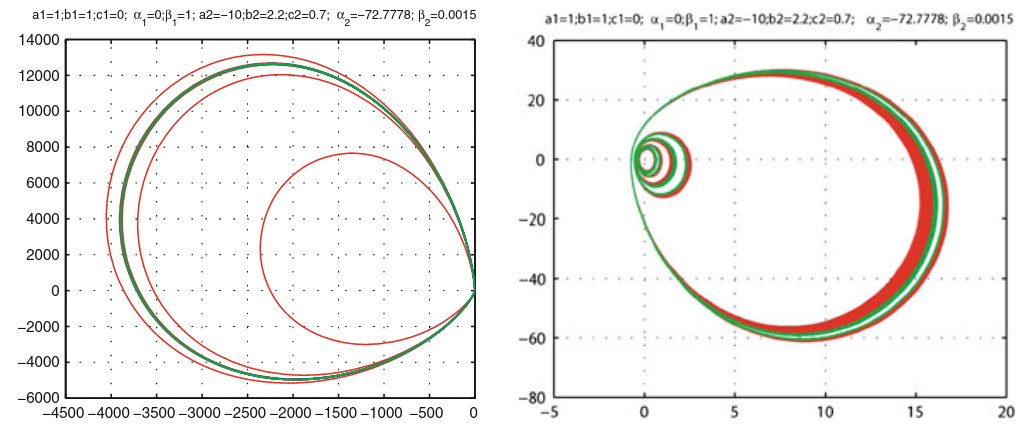
\includegraphics[width=1.0\textwidth]{4cycles}
    \caption{Visualization of four limit cycles in two-dimensional polynomial quadratic system, from Ref.~\cite{kuznetsov_visualization_2013}
    }%
    \label{fig:kuznetsov}
\end{figure}

To do so, we will implement an efficient parallel algorithm that solves systems
of ordinary differential equations (ODE) and detects limit cycles for a wide
range of parameters and points in the plane.  This code will be implemented in
Julia programming language and will use CUDA framework in such a way that
massive parallel calculation can be done on a dedicated CUDA server with several
advanced GPU graphic cards.

\pagebreak

\subsection{Computational complexity}

In~\cref{eq:system} we have 5 parameters for $x$ and 5 for $y$ which makes a
total of 10 distinct parameters. Adding the initial point to calculate the
trajectories ($x$ and $y$ coordinates) it makes a total of 12 parameters.
However we will only consider the reduced for of the system which only has 5
parameters (parameters for $x$ are 1) as shown in~\cref{eq:system2}. This gives
a total of 7 parameters.

\begin{align}\label{eq:system2}
    \frac{dx}{dt} &= x^2 + xy + y^2 + x + y \nonumber \\
    \frac{dy}{dt} &= a_2x^2 + b_2xy + c_2y^2 + \alpha_2x + \beta_2y
\end{align}


If we consider $n$ different values for each of those parameters we have a total
of $n^7$ different trajectories to calculate. If we were to compute the
trajectories sequentially it would take a long time for moderately sized values
of $n$. Calculating a trajectory on my machine takes 0.01 seconds. This means
that for $n=10$ it would take approximately 28 hours to compute all the
trajectories and taking $n=30$ the time increases to 7 years. If we use a GPU
with 5000 CUDA cores (Tesla K90) it would only take 20 seconds (assuming perfect
parallelization which is unrealistic). And for $n=30$ it would take 12 and a
half hours. If we consider the usage of a super computer like the Mare nostrum
with a cluster of 39 servers with 2 Tesla K90 GPUs the time for $n=30$ is a mere
9 minutes. \footnote{All these calculations are based on a very rough estimate
of the computing time needed to determine the limit cycle of a trajectory which
may vary a lot depending on the system and the implementation of the code}

\subsubsection{Stakeholders}

The main stakeholder in this project is the director Grigori Astrakharchik who
has a direct implication on the Thesis.

\pagebreak
\subsection{Justification}
\subsubsection{Previous studies}

In~\cite{kuznetsov_visualization_2013} there is a description of a task given by
the academician A.N. Kolmogorov:

\begin{quote}
To estimate the number of limit cycles of square vector fields on plane, A.N. Kolmogorov had
distributed several hundreds of such fields (with randomly chosen coefficients
of quadratic expressions) among a few hundreds of students of Mech \& Math
Faculty of Moscow State University as a mathematical practice. Each student had
to find the number of limit cycles of a field. The result of this experiment was
absolutely unexpected: not a single field had a limit cycle!
\end{quote}

This shows that the parallelizable nature of the problem and how difficult it is
to find those cycles. Therefore it is important to implement a code that is both
efficient on the calculation and have a big enough search space to find results.

There have been a number of studies relying on numerical methods to find limit
cycles in two dimensional vector fields
\cite{leonov_hidden_2013,van_der_hoff_numerical_2013,casades_computation_2013,gasull_effective_nodate}.
Papadimitriou and Vishnoi showed that the computation of a limit cycle is
% todo
% PSPACE??
\textbf{PSPACE}-complete~\cite{papadimitriou_computational_2015}.
The maximal known number of limit cycles is reported in Kuznetsov et
al.~\cite{kuznetsov_visualization_2013} where an example of specific conditions
for which 4 limit cycles is provided.

% todo

The CUDA framework has API for several programming languages (C, C++, Fortran,
Python, MATLAB, \dots). The official programming toolkit is in C/C++ and offers
the most customizability and low level configuration to adapt the code to the
hardware. The two most notable alternatives are Python's pyCUDA and Julia's
CUDA.jl libraries. These libraries bind to the C CUDA API and interface the data
between the kernels and the programming language. As such, the performance of
the kernels that run in the GPU should be equivalent in all cases but the data
models and processing of different languages makes a difference when interfacing
between the GPU code and the CPU code.

However, languages such as Python and Julia allow for faster coding and easier
visualization of the data. For this Thesis we will use Julia programming
language since it's faster than Python, has many libraries and tools for
numerical analysis and has type checking.  Nonetheless, this is not a strict
constraint and the possibility of writing specific C CUDA code to tweak the
performance to the maximum will be studied.

% There are various programming languages (C, C++, Fortran, Python and MATLAB) compatible with CUDA and which have libraries for CUDA programming.
%There are various programming languages with libraries for CUDA programming.
%In GPU-accelerated applications, the sequential part of the workload runs on the CPU – which is optimized for single-threaded performance – while the compute intensive portion of the application runs on thousands of GPU cores in parallel. When using CUDA, developers program in popular languages such as C, C++, Fortran, Python and MATLAB and express parallelism through extensions in the form of a few basic keywords.
%The official CUDA programming model is in C/C++ and offers the most flexibility and performance. The other two most notable alternatives are Python's Numba and Julia's CUDA.jl.
%These are higher-level libraries and
%are more limited in the versatility
%%do not offer the same low level options
%but allow easier development and visualization of the data.
%Both Python and Julia use the official CUDA C interface under the hood so
%although the performance is not as good as with pure C, if an appropriate
%realization of the methods is done, the performance might be still good if the
%majority of the work is done in the CUDA kernels. Since Julia JIT compilation is
%faster than the python's one and provides similar advantages when visualizing
%data the initial idea is to program the whole project in Julia programming
%language.


% todo

\pagebreak
\subsection{Scope}
\subsubsection{Objectives and sub-objectives}

The main objective of this Thesis is to develop a highly-efficient code capable
of determining the possible existence of limit cycles for a system. This code
must also be capable of being executed in parallel in a GPU cluster making full
use of its computing power to simulate a wide variety of systems with different
parameters. Furthermore, the results must be processed to find interesting
systems to visualize and analyse in more detail. These objectives can be divided
in sub-objectives:

\paragraph{Theoretical part}

Before implementing the algorithms and developing the code, a deep understanding
of the current numerical methods and the CUDA framework must be achieved to find
the best approach to the problem.

\begin{itemize}
    \item Explore the best strategies to solve ordinary differential equations.
    \item Explore numerical methods to verify the existence of limit cycles and determine the number of cycles for a given system.
    \item Research how these methods can be applied to run in a CUDA system efficiently.
\end{itemize}

\paragraph{Practical part} Having done the background research, the code must be
developed, implemented and tested.  Different methods will be tried in order to
find the ones that give the best performance.

\begin{itemize}
    \item Implement the algorithms in an efficient code.
    \item Benchmark the performance and compare different approaches to achieve the best performance.
    \item Run the code on a dedicated GPU server.
    \item Analyse the results and visualize them.
    \item Present and discuss the obtained results in the Thesis.
\end{itemize}

\subsubsection{Requirements}

To ensure the quality of the Thesis a number of requirements must be fulfilled:
\begin{itemize}
    \item Find the best balance between accuracy of the results and computational complexity
    \item Ensure that the numerical methods applied are properly implemented.
    \item Take into account numerical stability of the methods used as well as rounding and overflow errors.
    \item Profile the different methods under the same conditions and environment to ensure that there are no biases.
    \item Use good programming practices, making readable and maintainable code with the least complexity possible.
    \item Make the developed code publicly available.
\end{itemize}

\subsubsection{Potential obstacles and risks}

There are several risks that may have to be dealt with during the development of this Thesis.

\begin{itemize}
    \item \textbf{Project deadlines}: There is a limited amount of time to do
        the project. Therefore, a proper planning of tasks and time must be made
        and followed to ensure that the work can be done in the proper time
        frame.
    \item \textbf{Computational power}: This Thesis involves a lot of
        computational power and the whole project is conditioned by it. If the
        program cannot be run on the proper hardware the results may not be
        obtainable in a realistic time frame and the scope of the project will
        have to be reevaluated.
    \item \textbf{Inexperience on the field}: I have very limited experience
        with CUDA programming and just the basics of numerical computation
        techniques so there is a lot of research to be done, specially regarding
        dynamical systems.
\end{itemize}

\pagebreak
\subsection{Methodology and rigor}

\subsubsection{Methodology}

Since the Thesis must be completed in a relatively short period of time we will
apply the \emph{agile} methodology and divide the work into sub-tasks or
\emph{sprints}. These \emph{sprints} will consist of different stages of
implementation of the program, beginning with a proof of concept running in
sequence on the CPU and progressively iterating on this base to optimize the
methods and adapt them to be able to run in CUDA on the GPU.

\subsubsection{Monitoring tools and validation}

To manage the different iterations of the code \texttt{git} will be used. The
repository will be hosted on \emph{GitHub} and access will be granted to the
project tutor allowing him to follow and monitor the work and results at any
time.

A weekly meeting with the tutor will be arranged to discuss the progress and
which tasks should be worked on.

    %! TEX root = **/010-main.tex
% vim: spell spelllang=en:

\section{Time planning}

The work-to-begin date is on February 9th and the delivery date on June which
gives around 18 weeks of time. I plan to work on the project approximately 35
hours a week, this gives around 630 hours in total working on the project.

\subsection{Description of the tasks}

\subsubsection{Task definition}

The definitions of the tasks that will be done throughout the project are
divided into 4 categories: planning, research, implementation and experimentation.

\paragraph{Project planning}

\begin{itemize}
    \item \textbf{Contextualization and project scope} Describe the project
        scope and its context. Giving an overview of the objective, other past
        studies on the topic and how this project is relevant.
    \item \textbf{Time planning} Organize the work to be done in granular tasks
        to estimate the time needed for each of them. With the time estimation
        create a realistic planning for the tasks completions so that the
        project can be finished in the appropriate time frame.
    \item \textbf{Budget and sustainability} Analyze the economic and
        environmental sustainability of the project.
    \item \textbf{Meetings} Each week a meeting with the tutor will be scheduled
        to ensure that the thesis is proceeding correctly and within the
        expected deadlines.
    \item \textbf{Integration into the final document} All these project
        planning tasks must be integrated into the final thesis memoir.
\end{itemize}

\paragraph{Research}

Given the nature of this thesis it is fundamental to have a solid understanding
of modern numerical computation techniques applied to solving Ordinary
Differential Equations and finding limit cycles. It is also primordial to know
how these techniques can be applied to CUDA and how to benchmark the programs to
detect bottlenecks and find whether or not the processing power of the GPU is
being used in its full potential.

\begin{itemize}
    \item \textbf{Research ODE solvers} There are lots of algorithm to solve
        ODEs which will have to be tried to find the ones that give the best
        results in our case.
    \item \textbf{Research how to find limit cycles} Find the best approach to
        detect limit cycles
    \item \textbf{Research CUDA} This task includes reading the official
        documentation as well as other sources on numerical methods applied to
        CUDA.
\end{itemize}

\paragraph{Practical Implementation}

The different algorithms researched must be implemented in order to experiment
with them and find the best ones to solve the problem.

\begin{itemize}
    \item \textbf{Program different methods to find limit cycles} As stated
        before various different methods will have to be implemented. This
        implementation can be initially without using CUDA (fully sequential).
    \item \textbf{Adapt de code to be run with CUDA} Once the methods to find
        limit cycles are properly implemented they must be adapted in order to
        be run with CUDA.
    \item \textbf{Test the program} In order to ensure that the code implemented
        is correct and the errors introduced in the computation fall within a
        reasonable distance of the real theoretical value some tests must be
        implemented. This includes also the implementation of small programs to
        visualize the results and interpret them.
\end{itemize}

\paragraph{Experimentation, analysis and conclusions}

Once there is a working prototype of the code the experimentation can begin.
There will be two major parts of the experimentation, the first one when the
various methods are tested with a relatively small number of cases to find the
best one (taking into account both the speed and accuracy of the calculations)
and the final experiment when the best method is run with a much bigger search
space and from which the results can be analysed.

\begin{itemize}
    \item \textbf{Comparison experiment}
        \begin{itemize}
            \item \textbf{Select search space} Decide how many different
                parameters will be used on the experiment. It should be a big
                enough search space so as to have variety on the systems but not
                big enough that it takes too much time to benchmark and slows
                down the development.
            \item \textbf{Select benchmarks} The benchmarks must be run in
                similar conditions and we must decide what metrics will be
                considered (runtime, GFLOPS, accuracy, \dots).
            \item \textbf{Further optimize the methods} When running the
                benchmarks we may find some possible improvements on the
                original implementations which can then be improved and tested
                again.
            \item \textbf{Analyse results and decide best method} With the
                results of the experiments we can decide on which method is the
                best and should therefore be used in the final experiment.
        \end{itemize}
    \item \textbf{Final experiment}
        \begin{itemize}
            \item \textbf{Select search space} Given the results of the previous
                experiments, estimate the runtime as a function of the search
                space and select a search space as big as possible given the
                available computing time.
            \item \textbf{Analyse results} Once the final experiment finishes
                the results can be analysed in search of systems with
                interesting number of limit cycles.
        \end{itemize}
    \item \textbf{Conclusions} Analyse the results of both experiments and
        provide a conclusion.
\end{itemize}

\pagebreak
\subsubsection{Summary of the tasks}

\begin{table}[H]
    \centering
    \caption{Summary of tasks}
    \begin{tabular}{llrc}
        \toprule
        \thead{ID} & \thead[l]{Task} & \thead{Time (h)} & \thead{Depend.} \\
        \midrule
    \texttt{P} & \textbf{Project planning} & \textbf{60} & \\
        \texttt{P0} & - Contextualization and project scope & 10 & \\
        \texttt{P1} & - Time planning & 10 & \\
        \texttt{P2} & - Budget and sustainability & 10 & \\
        \texttt{P3} & - Meetings & 18 & \\
        \texttt{P4} & - Integration into final document & 12 & \\

        \addlinespace[0.5em]
    \texttt{R} & \textbf{Research} & \textbf{150} & \\
        \texttt{R0} & - ODE solvers & 50 & \\
        \texttt{R1} & - Limit cycles & 50 & \\
        \texttt{R2} & - CUDA & 50 & \\

        \addlinespace[0.5em]
    \texttt{I} & \textbf{Implementation} & \textbf{200} & \\
        \texttt{I0} & - Different methods to find limit cycles & 100 & \texttt{R0,R1} \\
        \texttt{I1} & - Adapt to CUDA & 50 & \texttt{I0,R2} \\
        \texttt{I2} & - Tests & 50 & \\

        \addlinespace[0.5em]
    \texttt{EC} & \textbf{Experimentation (comparison)} & \textbf{130} & \texttt{I} \\
        \texttt{EC0} & Select search space & 5 & \\
        \texttt{EC1} & Select benchmarks & 5 & \\
        \texttt{EC2} & Further optimize the methods & 100 & \\
        \texttt{EC3} & Analyse the results and decide the best method & 20 & \\

    \addlinespace[0.5em]
    \texttt{EF} & \textbf{Experimentation (final)} & \textbf{25} & \texttt{EC} \\
        \texttt{EF0} & Select search space & 5 & \\
        \texttt{EF1} & Analyse the results & 20 & \\

    \addlinespace[0.5em]
        \texttt{C} & \textbf{Conclusions} & \textbf{10} & \texttt{EC,EF} \\
        \texttt{D} & \textbf{Documentation} & \textbf{60} & \\
        \texttt{O} & \textbf{Oral exposition} & \textbf{10} & \\
        \bottomrule
    \end{tabular}
\end{table}
% table

\pagebreak
\subsubsection{Resources}

\paragraph{Human resources}

The main human resource of the thesis is the researcher.  There is also the
director Grigori Astrakharchik which mentors the researcher and the GEP Tutor
Eguiguren Huerta Marcos in charge of correcting the project management part.

\paragraph{Material resources}

The main resources needed for this project are previous papers and books on the
topics of ODEs, limit cycles and CUDA. For the implementation an execution of
the code there following resources will be used:

\begin{itemize}
    \item \textbf{VCS}: \texttt{git} will be used as a version control
        system~(VCS) and the code will be hosted on \emph{GitHub} for easy
        collaboration with the director.
    \item \textbf{\LaTeX}: To format the document \LaTeX will be used. The
        document will be hosted on \emph{Overleaf} to allow easier collaboration
        and due to the fact that it provides \emph{github} integration.
    \item \textbf{Atenea}: To communicate with the GEP tutor.
    \item \textbf{Computers}: My own personal computer with an \emph{RTX2060} will be
        used to develop the code and test it. The final versions will will run
        on a server from the department of physics at UPC with a \emph{Nvidia
        Titan V} and \emph{Nvidia Titan Xp} GPUs.
    \item \textbf{Julia}: The Julia programming language will be used to write
        the code and visualize the results.
\end{itemize}

%! TEX root = **/010-main.tex
% vim: spell spelllang=en:

\newgeometry{top=0.5cm, bottom=0.5cm, left=0.5cm, right=0.5cm}
\thispagestyle{empty}
\begin{landscape}
\subsection{Gantt chart}

\begin{figure}[H]
\centering
\resizebox{28cm}{!}{%
\begin{ganttchart}[
vgrid={*{6}{draw=none}, dotted},
x unit=.40cm,
y unit title=1cm,
y unit chart=1cm,
    time slot format=isodate
    ]{2021-02-09}{2021-06-07}
\gantttitlecalendar{month=name, day}
\ganttnewline

\ganttgroup{Project planning}{2021-02-09}{2021-03-22}
\ganttnewline
\ganttbar{Contextualization and scope}{2021-02-23}{2021-03-02}
\ganttnewline
\ganttbar{Time planning}{2021-03-02}{2021-03-09}
\ganttnewline
\ganttbar{Budget and sustainability}{2021-03-09}{2021-03-16}
\ganttnewline
\ganttbar{Integration into final document}{2021-03-16}{2021-03-22}
\ganttnewline

\ganttgroup{Research}{2021-02-09}{2021-04-01}
\ganttnewline
\ganttbar{ODE Solvers}{2021-02-09}{2021-03-02}
\ganttnewline
\ganttbar{Limit cycles}{2021-02-16}{2021-03-09}
\ganttnewline
\ganttbar{CUDA}{2021-03-09}{2021-03-22}
\ganttnewline

    % \texttt{R} & \textbf{Research} & \textbf{150} & \\
    %     \texttt{R0} & - ODE solvers & 50 & \\
    %     \texttt{R1} & - Limit cycles & 50 & \\
    %     \texttt{R2} & - CUDA & 50 & \\

\ganttgroup{Implementation}{2021-02-22}{2021-05-02}
\ganttnewline
\ganttbar{Find limit cycles}{2021-02-22}{2021-04-01}
\ganttnewline
\ganttbar{Adapt to CUDA}{2021-04-01}{2021-05-02}
\ganttnewline
\ganttbar{Tests}{2021-03-09}{2021-05-02}
\ganttnewline

    %     \addlinespace[0.5em]
    % \texttt{I} & \textbf{Implementation} & \textbf{200} & \\
    %     \texttt{I0} & - Different methods to find limit cycles & 100 & \texttt{R0,R1} \\
    %     \texttt{I1} & - Adapt to CUDA & 50 & \texttt{I0,R2} \\
    %     \texttt{I2} & - Tests & 50 & \\

\ganttgroup{Experimentation (comparison)}{2021-04-05}{2021-05-16}
\ganttnewline
\ganttbar{Select search space}{2021-04-05}{2021-04-06}
\ganttnewline
\ganttbar{Select benchmarks}{2021-04-05}{2021-04-06}
\ganttnewline
\ganttbar{Further optimizations}{2021-04-07}{2021-05-01}
\ganttnewline
\ganttbar{Analyse results}{2021-05-01}{2021-05-16}
\ganttnewline

    %     \addlinespace[0.5em]
    % \texttt{EC} & \textbf{Experimentation (comparison)} & \textbf{130} & \texttt{I} \\
    %     \texttt{EC0} & Select search space & 5 & \\
    %     \texttt{EC1} & Select benchmarks & 5 & \\
    %     \texttt{EC2} & Further optimize the methods & 100 & \\
    %     \texttt{EC3} & Analyse the results and decide the best method & 20 & \\

\ganttgroup{Experimentation (final)}{2021-05-16}{2021-05-30}
\ganttnewline
\ganttbar{Select search space}{2021-05-16}{2021-05-17}
\ganttnewline
\ganttbar{Run experiment}{2021-05-17}{2021-05-25}
\ganttnewline
\ganttbar{Analyse results}{2021-05-25}{2021-05-30}
\ganttnewline

    % \addlinespace[0.5em]
    % \texttt{EF} & \textbf{Experimentation (final)} & \textbf{25} & \texttt{EC} \\
    %     \texttt{EF0} & Select search space & 5 & \\
    %     \texttt{EF1} & Analyse the results & 20 & \\

\ganttgroup{Project Documentation}{2021-02-09}{2021-06-07}
\ganttnewline
\ganttbar{Documentation}{2021-02-09}{2021-06-07}
\ganttnewline
\ganttbar{Conculsions}{2021-05-25}{2021-06-04}
\ganttnewline
\ganttbar{Oral exposition}{2021-06-01}{2021-06-07}
\ganttnewline
    % \addlinespace[0.5em]
    %     \texttt{C} & \textbf{Conclusions} & \textbf{10} & \texttt{EC,EF} \\
    %     \texttt{D} & \textbf{Documentation} & \textbf{60} & \\
    %     \texttt{O} & \textbf{Oral exposition} & \textbf{10} & \\

\end{ganttchart}
}

\caption{Gantt chart}%
\label{fig:gantt}
\end{figure}

\end{landscape}
\restoregeometry


\subsection{Risk Management}

% todo link with intro section

    \subsubsection{Project deadline}
    There is the possibility that the initial estimation made of the time it takes to
    complete each task was wrong due to unexpected difficulties. Therefore it's
    crucial that there is enough time to accommodate possible delays and that
    these setbacks are detected immediately and taken into account (Possibly
    redoing the initial time planning).

    \subsubsection{Computational power}
    The program will be run in a server of the department of physics of UPC.
    Although it should not be a problem in the event of not being able to use
    that computing power the code can be run locally on my own GPU (this will
    take much longer time).

    \subsubsection{Inexperience on the field}
    Sine I have limited experience with both CUDA and numerical computation of
    ODEs there is a significant amount of hours dedicated to studying the
    concepts and researching numerical methods.

    %! TEX root = **/010-main.tex
% vim: spell spelllang=en:

% \addtocontents{toc}{\protect\pagebreak}

\section{Budget}%
\label{sec:budget}

\subsection{Staff costs}%
\label{sub:staff}

Although the tasks in the project are going to be performed by me and the tutors
I will break them down into different roles in order to estimate the cost of the
project. We will have a \textbf{Project manager} responsible of planning the
project. A \textbf{Junior researcher} that will study the different
computational methods and techniques needed to perform the calculations in the
project. The \textbf{Junior developer} will implement the code according to the
instructions given by the researcher and this code will be tested by a
\textbf{Tester} to ensure that the implementation is correct. Finally a
\textbf{Technical writer} will compile all the results obtained and write the
final document.

Using data from \url{https://www.payscale.com} we can estimate the cost of the
different roles that take part in the project as shown in~\cref{tab:pay}. With
these estimations we can calculate the overall cost of the staff in the project
which is shown in~\cref{tab:cost}.

\begin{table}[H]
    \centering
    \caption{Cost per hour of different roles}\label{tab:pay}
    \begin{tabular}{lr}
        \toprule
        \thead{Role} & \thead{Cost (€/h)} \\
        \midrule
        Project manager & 23 \\
        Junior developer & 15 \\
        Junior researcher & 22 \\
        Tester & 8 \\
        Technical writer & 13 \\
        \bottomrule
    \end{tabular}
\end{table}

\begin{table}[H]
    \centering
    \caption{Total cost of tasks}\label{tab:cost}
    \begin{tabular}{lrcr}
        \toprule
    \thead{Task} & \thead{Time \\ (h)} & \thead{Role\footnotemark} & \thead{Cost \\ (€)} \\
        \midrule
    \textbf{Project planning} & \textbf{60} & PM & \textbf{1,380} \\
        % - Contextualization and project scope & 10 & \\
        % - Time planning & 10 & \\
        % - Budget and sustainability & 10 & \\
        % - Meetings & 18 & \\
        % - Integration into final document & 12 & \\

        \addlinespace[0.5em]
        \textbf{Research} & \textbf{150} & JR & \textbf{3,300}\\
        % - ODE solvers & 50 & \\
        % - Limit cycles & 50 & \\
        % - CUDA & 50 & \\

        \addlinespace[0.5em]
        \textbf{Implementation} & \textbf{200} & JD,T & \textbf{2,650} \\
        - Different methods to find limit cycles & 100 & JD & 1500 \\
        - Adapt to CUDA & 50 & JD & 750 \\
        - Tests & 50 & T & 400 \\

        \addlinespace[0.5em]
        \textbf{Experimentation (comparison)} & \textbf{130} & JR,JD & \textbf{2,160} \\
        - Select search space & 5 & JR & 110 \\
        - Select benchmarks & 5 & JR & 110 \\
        - Further optimize the methods & 100 & JD & 1500 \\
        - Analyse the results and decide the best method & 20 & JR & 440 \\

    \addlinespace[0.5em]
        \textbf{Experimentation (final)} & \textbf{25} & JR & \textbf{550} \\
        % Select search space & 5 & \\
        % Analyse the results & 20 & \\

    \addlinespace[0.5em]
        \textbf{Conclusions} & \textbf{10} & W & \textbf{130} \\
        \textbf{Documentation} & \textbf{60} & W & \textbf{780}\\
        \textbf{Oral exposition} & \textbf{10} & W & \textbf{130} \\
    \addlinespace[1em]
        \textbf{Total} & & & \textbf{11,080} \\

        % 1380
        % 3300
        % 2650
        % 2160
        % 550
        % 130
        % 780
        % 130
        \bottomrule
    \end{tabular}
\end{table}

\footnotetext{PM = Project Manager, JR = Junior Researcher, JD = Junior
Developer,\\ W = Technical Writer}

% \begin{table}[H]
%     \centering
%     \caption{Total cost of the staff}
%     \begin{tabular}{cc}
%         \toprule
%         Role & Cost (€) \\
%         \midrule
%         Project manager & 23 \\
%         Junior developer & 15 \\
%         Junior researcher & 22 \\
%         Tester & 8 \\
%         Technical writer & 13 \\
%         Total & \\
%         \bottomrule
%     \end{tabular}
% \end{table}


\pagebreak
\subsection{Generic costs}

% Other than the staff costs, there are other cost that must be taken into
% account.

\subsubsection{Amortization of the resources}

I will work approximately 3.7 hours per day during 130 days. Most of the time on
my Lenovo laptop (80\%) and the rest on an HP laptop which is more lightweight
and can be carried around easily. Using the formula to compute the
amortization~(\cref{eq:amort}) we obtain the \cref{table:amort} which shows the
amortization of the hardware used.

\begin{equation}\label{eq:amort}
    \text{Amortization} = \text{Price} \times \frac{1}{\text{Years of use}}
    \times \frac{1}{\text{Days of work}} \times \frac{1}{\text{Hours per day}}
    \times \text{hours used}
\end{equation}

\begin{table}[H]
    \centering
    \caption{Amortization of hardware}\label{table:amort}
    \begin{tabular}{lrcr}
        \toprule
        \thead{Hardware} & \thead{Cost \\ (€)} & \thead{Life expectancy \\
        (years)} & \thead{Amortization \\ (€)} \\
        \midrule
        Lenovo laptop & 1,400 & 6 & 211.89 \\
        HP laptop & 600 & 4 & 28.38\\
        \addlinespace[0.5em]
        \textbf{Total} & \textbf{2,000} &   & \textbf{240.27} \\
        \bottomrule
    \end{tabular}
\end{table}

\subsubsection{Indirect costs}

A part from the hardware costs of the laptops there are more indirect costs that
must be considered:

\begin{itemize}
    \item \textbf{Internet:} With an internet cost of 100€ per month during 5
        months working 3.7 hours per day the total is: $100€ \cdot 5 \cdot
        \nicefrac{3.7}{24} = 77.08€$.
\item \textbf{Electricity} Given a cost of \SI{0.1270}{€\per\kWh} and the fact that
    my Lenovo laptop consumes \SI{230}{\watt} at peak performance (which should
        happen rarely) we can estimate the electricity cost as:
    $\SI{0.1270}{€\per\kWh} \cdot \SI{0.230}{\kW} \cdot 0.5 \cdot \SI{630}{\hour} = 9.21€$.
\end{itemize}

In total there are $86.29€$ of indirect costs which, added to the hardware
amortization, result in $326.56€$ of generic costs.

\subsection{Contingency}

During the development of the project unforeseen events may occur that may
impact our budget. Therefore a 15\% increase on the total cost will be added as
a contingency margin. Given that the Cost per Action ($CPA$) is $11,080€$
and the Generic Costs ($GC$) are $326.56€$ for a total of $11,406.56€$. The contingency
budget is then $1710.99€$.

\subsection{Incidental costs}

The following table estimates the cost of the different incidents that may
impact the project given their estimated cost and the risk that they happen.

\begin{table}[H]
    \centering
    \caption{Incidental costs}\label{tab:inc}
    \begin{tabular}{lrrr}
        \toprule
        \thead{Incident} & \thead{Estimated Cost (€)} & \thead{Risk (\%)} & \thead{Cost (€)} \\
        \midrule
        Project deadline & 500 & 25 & 125 \\
        Computational power & 100 & 50 & 50 \\
        Inexperience on the field & 300 & 25 & 75 \\
        \addlinespace[0.5em]
    \textbf{Total} & \textbf{900} & & \textbf{250} \\
        \bottomrule
    \end{tabular}
\end{table}


\subsection{Final budget}

\begin{table}[H]
    \centering
    \caption{Final budget}\label{tab:final}
    \begin{tabular}{lr}
        \toprule
        \thead{Activity} & \thead{Cost (€)} \\
        \midrule
        $CPA$ & 11,080.00 \\
        $GC$ & 326.56 \\
        Contingency & 1,710.98 \\
        Incidental cost & 250.00 \\
        \addlinespace[0.5em]
        \textbf{Total} & \textbf{13,367.54} \\
        \bottomrule
    \end{tabular}
\end{table}

\pagebreak
\subsection{Management control}

In the previous section there is an estimation of the budget and its potential risks and
incidents along with their impact. We also need a model to detect the
deviation on these initial budget estimations. Upon finishing a task $t$, we will
calculate its deviation:

\begin{equation}
    d_t = E_t - R_t
\end{equation}

Where:

\begin{itemize}
    \item $E_t = $ \textbf{Estimated cost} of the task on the initial budget
        plan
    \item $R_t = $ \textbf{Real cost} of the task when finished. Here we have to
        recalculate the $CPA$, $GC$, Contingency and Incidents for the task.
    \item $d_t = $ \textbf{Deviation from initial cost:} this estimates how much
        we have deviated from the original budget for each task.
\end{itemize}

If $d_t$ is negative I will reallocate the extra money for future incidents, if
it's positive some of the funds for contingency will be used to cover the costs.
If the contingency funds are not enough the whole budget planning will be
readdressed.

To keep track of this deviances from the budget a budget spreadsheet will be
used. This spreadsheet will contain all the information on the tasks, their
estimated cost, the real cost and the deviation calculations. All this budget
data will be kept up to date and updated every time a task is finished. When the
data is updated the deviation will immediately be apparent and the
aforementioned steps will be taken.

\pagebreak
\section{Sustainability}%
\label{sec:sustainability}

\subsection{Self-assessment}

Before starting the sustainability assessment I did not know how many indicators
and factors must be taken into account when doing a sustainable project. I had
not considered the impact that project a part from the immediate actors involved
in it. Through this assessment I realized how the project can impact the
environment, the society and the economy in ways I had not thought about before.

\subsection{Environmental impact}

\subsubsection*{Regarding PPP, Have you estimated the environmental impact of
undertaking the project? Have you considered how to minimise the impact, for
example by reusing resources?}

The main impact of this project on the environment is the use of computer
resources and therefore electric power to do the complex calculations needed.
The aim of the project is not only to develop a program that works but that it
also uses the least amount of resources so that it does not waste computing
power. In order to avoid wasting resources, only the final version will be run
on a big search space and during development the tests will be on a much reduced
search space.

\subsubsection*{Regarding the life expectancy, How is the problem that you wish
to address resolved currently (state of the art)? In what ways will your
solution environmentally improve existing solutions?}

Currently there is not much work on the research of the number of limit cycles
in second degree ODEs and the current approaches rely on heady computations in
order to calculate the cycles. With this new approach the aim is to search with
a faster implementation although less accurate which will hopefully find
interesting systems that can then be analyzed in more detail.


\pagebreak
\subsection{Economy}

\subsubsection*{Regarding PPP, Have you estimated the cost of undertaking the
project (human and material resources)?}

In~\cref{sec:budget} there is a description of the cost of the project taking
into account human and material resources as well as potential risks and
contingencies.

\subsubsection*{Regarding the life expectancy, How is the problem that you wish
to address resolved currently (state of the art)? In what ways will your
solution economically improve existing solutions?}

As stated on the Sustainability section, if a faster more efficient method to
identify limit cycles is implemented it will reduce the amount of computational
power needed and therefore the resources.


\subsection{Social}

\subsubsection*{Regarding PPP, What do you think undertaking the project has
contributed to you personally?}

The project enables me to research on various topics that interest me and has
given me a new view on the applications of GPUs for scientific research.

\subsubsection*{Regarding the life expectancy, How is the problem that you wish
to address resolved currently (state of the art)? In what ways will your
solution socially improve (quality of life) existing Is there a real need for
the project?}

The nature of this project as a research project on the field of dynamical
systems does not have a direct impact on the society as a whole. However if
interesting results are obtained it could bring some insight into Hilbert 16th
problem which has remained unsolved for more than a century.


    %! TEX root = **/010-main.tex
% vim: spell spelllang=en:

\section{Program structure}%
\label{sec:structure}

Initially, all the program was to be implemented in pure \emph{Julia} since there are libraries to interface with \emph{CUDA} \cite{noauthor_juliagpu_nodate} that should be able to handle the tasks needed. However there were some complications with the \emph{Nvidia} drivers and compiling the \emph{Julia} \emph{CUDA} kernels and some features are not yet available in \emph{CUDA.jl}.

Therefore, the main program in \emph{CUDA} will be implemented in \emph{C} and expose the relevant method through an \emph{ABI} (Application Binary Interface) so that it can be compiled into a shared binary and interface with \emph{Julia} or any other language capable of using \emph{C} shared libraries. With this approach we can achieve seamless interoperation between \emph{CUDA} and \emph{Julia} while having full control of how \emph{CUDA} kernels behave and manage the resources. All the analysis on the data obtained from the \emph{CUDA} computation can then be processed using all the available \emph{Julia} libraries offering great flexibility.

The \emph{ABI} interface will be very simple, exposing a method to initialize the GPU memory, and the various different kernels to compute the data and transfer the result to \emph{Julia}. Since \emph{Julia} is able to use \emph{C} structures natively through
its \emph{C} interface there is no overhead when transferring data since pointers can be shared \cite{noauthor_c_nodate} and all the memory management can be delegated
to \emph{C}.

% \begin{figure}[H]
%     \centering
% \begin{tikzpicture}[node distance=2.5cm,auto,>=latex']
%     \node[draw, circle] (C) at (0,0){C};

% \node [draw, right=1cm of C]  (gpu) {GPU};

% \node [draw, circle, left=1cm of C]  (julia) {Julia};

% \draw[-stealth] (julia.east) -- (C.west)
%     node[midway,above]{run};
% \draw[-stealth] (C.east) -- (gpu.west)
%     node[midway,above]{run kernel};

% \end{tikzpicture}
% \caption{ABI diagram}
% \end{figure}


\pagebreak
\section{Initial implementation}%
\label{sec:initial_implementation}

Before implementing the program in CUDA we first need to implement a sequential version of the program. This sequential code allows easier debugging of the implementation and provides a basis to compare the speedup obtained with CUDA.

The main steps that the program must perform are:

\begin{enumerate}
    \item Compute a trajectory starting at various different points.
    \item Determine if the trajectory is a limit cycle.
    \item Classify all the starting points into groups corresponding to
        the different limit cycles.
\end{enumerate}

The first two steps of computing the trajectory and determining if it is a limit cycle will be parallelized using \emph{CUDA} and the last step of analysis will be done using \emph{Julia}.

\subsection{Computing the trajectory}

To compute the trajectory, a numerical method to integrate an ODE must be used. There are various methods that can be used with varying complexity. In the program we implemented \emph{Runge-Kutta} methods of different order [1, 2, (2)3, 4 and 4(5)] \cite{butcher_numerical_2008}. Two of these methods allow for adaptive time stepping [(2)3 and 4(5)] meaning that they adjust the time steps ($h$) according to the error tolerance.

There is no need to save all the trajectory to detect the cycles since the relevant metrics can be computed as the integration step is happening. This reduces not only the amount of memory needed to compute and store the results but also allows the early termination of a trajectory computation if we detect that it is a cycle, point or it goes out of bounds before the last step is reached.

In~\cref{sec:metrics} there is an in-depth discussion of the metrics used and how they are used to find limit cycle candidates. For the moment the relevant point is that for each trajectory we only need to compute 2 \emph{loops} and measure the ratio between the maximum and minimum points of each loop. If this ratio is equal to 1 (within a tolerance margin), the trajectory is a cycle.

\paragraph{Julia}
For the very first prototyping, the various methods where implemented in \emph{Julia}
to check the correctness of the algorithm and then manually translated into \emph{C}
and checked again.

\paragraph{C translation}

In \cref{lst:julia_rk4,lst:c_rk4} we can see the main RK4 routine implemented in \emph{Julia} and the corresponding \emph{C} translation. Both versions of all methods were tested to ensure that they where properly implemented (In~\cref{sec:convergence} there is a detail comparison of the accuracy of the methods).

% Julia -> C


\begin{listing}[H]
    \caption{Julia version of RK4 step}
    \label{lst:julia_rk4}
\begin{minted}{julia}
function RK4(f::Function, x, y, h)
    xk1, yk1 = h.*f(x, y)
    xk2, yk2 = h.*f(x + xk1/2, y + yk1/2)
    xk3, yk3 = h.*f(x + xk2/2, y + yk2/2)
    xk4, yk4 = h.*f(x + xk3, y + yk3)

    x = x + (xk1 + 2xk2 + 2xk3 + xk4)/6
    y = y + (yk1 + 2yk2 + 2yk3 + yk4)/6

    x, y
end
\end{minted}
\end{listing}

\begin{listing}[H]
    \caption{C version of RK4}
    \label{lst:c_rk4}
\begin{minted}{c}
__device__ void rk4_step(const double x0, const double y0, double *const x1, double *const y1, const double h, const double P[PARAMS]) {
    double cache[4][2];

    // xk1, yk1 = h.*f(x, y)
    f(x0, y0, h, &cache[0][0], &cache[0][1], P);

    // xk2, yk2 = h.*f(x + xk1/2, y + yk1/2)
    *x1 = x0 + cache[0][0]/2.0;
    *y1 = y0 + cache[0][1]/2.0;
    f(*x1, *y1, h, &cache[1][0], &cache[1][1], P);

    // xk3, yk3 = h.*f(x + xk2/2, y + yk2/2)
    *x1 = x0 + cache[1][0]/2.0;
    *y1 = y0 + cache[1][1]/2.0;
    f(*x1, *y1, h, &cache[2][0], &cache[2][1], P);

    // xk4, yk4 = h.*f(x + xk3, y + yk3)
    *x1 = x0 + cache[2][0];
    *y1 = y0 + cache[2][1];
    f(*x1, *y1, h, &cache[3][0], &cache[3][1], P);

    // x = x + (xk1 + 2xk2 + 2xk3 + xk4)/6
    // y = y + (yk1 + 2yk2 + 2yk3 + yk4)/6
    *x1 = x0 + (cache[0][0] + 2*cache[1][0] + 2.0*cache[2][0] + cache[3][0])/6.0;
    *y1 = y0 + (cache[0][1] + 2*cache[1][1] + 2.0*cache[2][1] + cache[3][1])/6.0;
}
\end{minted}
\end{listing}

% Sample code

    %! TEX root = **/010-main.tex
% vim: spell spelllang=en:

\section{Convergence analysis}%
\label{sec:convergence}

\begin{figure}[H]
    \centering
    \includegraphics[width=1.0\textwidth]{figures/plots/error_analysis/error_cycle.tikz}
    \caption{Integration error after one period with commensurate $\Delta t$}%
    \label{fig:error_cycle}
\end{figure}

\begin{figure}[H]
    \centering
    \includegraphics[width=1.0\textwidth]{figures/plots/error_analysis/error_pi.tikz}
    \caption{Error on the period estimation using interpolation}%
    \label{fig:error_pi}
\end{figure}


    %! TEX root = **/010-main.tex
% vim: spell spelllang=en:

\section{Metrics}%
\label{sec:metrics}

As discussed in previous sections, there is no need to save the full trajectory in order to detect limit cycle candidates; we can evaluate the trajectory's characteristics in-place.

To do so we have to detect special points in the trajectory that we can use to detect if we are in a cycle. These points must be easy to identify (computationally cheap) and should be present in all trajectories. By comparing the values of these points at each loop of the cycle we can estimate the behaviour of the trajectory.

\paragraph{Zero crossings:} can be computed by detecting the change of sign
during the computation. Although they are really cheap and are commonly used on complex ODE systems, there is no guarantee that cycles will cross axis.

\paragraph{Inflection points:} these correspond to the points where the ratio of change of the function changes sign (maxima, minima or stationary points). Given that the integration methods used compute the result as the previous value plus a change, we can easily detect changes in sign with almost no overhead. Moreover, all cycles will have at least four local extrema.

\paragraph{Interpolation:} although we can detect if we passed an inflection point with almost no overhead, we must perform some kind of interpolation to obtain an accurate value within our tolerances. To do so, we can perform interpolation using 3 neighbouring points or perform additional integration steps to find the inflection point numerically. Applying polynomial interpolation requires saving at least 3 point for each trajectory, interpolating them and computing the vertex. The second option (root finding) is potentially more costly since it involves additional integration steps but should produce better results.

\pagebreak

\subsection{Rate of change of extrema}%
\label{sub:roc}

Comparing the value of the initial 4 local extrema with the local extrema of the second loop of the cycle we can obtain a rate of change of the trajectory. For instance, given the values of the 4 local extrema on obtained on the first loop: $x_{\min}, x_{\max}, y_{\min}, y_{\max}$ and their counterparts obtained on the second loop: $x'_{\min}, x'_{\max}, y'_{\min}, y'_{\max}$ we can compute the ratio between each of them to obtain their rate of change. If the ratio is less than 1, the trajectory is \emph{decreasing}, if it is greater than 1 it is \emph{increasing} and if it is 1 (within an adequate tolerance) the trajectory is a cycle.

There is one small caveat with this approach which is that the ratios between the 4 different extrema are not comparable, that is, in some cases the maxima or minima are various orders of magnitude apart. This has to be taken into consideration when evaluating the values used for the tolerance when searching the points with ratio 1.

Traditionally with CPU computation one initial point is taken and evaluated through many steps until the trajectory reaches a stable cycle. Instead, the advantage of GPU computation is that one can take a massive amount of points, evaluate only the very few first steps (until 2 loops are completed) and quickly find limit cycle candidates.

\subsection{Other metrics}

Apart from the rate of change in local extrema, an evaluation of the rate of
change in the loop period was also attempted, but it did not give satisfying
results.

\subsection{Distinguishing different cycles}

The rate of change of extrema allows us to find areas in the function with
trajectories with a rate of change of their extrema of 1 (\cref{sub:roc}),
which are candidates to be limit cycles. Now the problem is how we can classify
these areas into different limit cycle trajectories. The following approaches
were tested:

\subsubsection*{Connected component labelling}

Connected component labelling is a technique often used in the field of computer vision. It consists of finding connected components in a graph and labeling each pixel according to the component in which they belong \cite{shapiro_connected_1996}.

Since the final result of our computation is a matrix with ones and zeros indicating the coordinates close to trajectories with rate of change 1, we have a binary image in which we can apply this technique. Ideally the connected components found will match the limit cycles, but there are two main caveats: there may be areas where resolution is not high enough (the discretization of the section was too big to and the points sampled missed the trajectory) and the line can be partially broken, thus splitting a cycle into two or more parts. The second problem appears when two cycles pass really close to each other and be classified as the same group. Therefore, this technique requires very small discretization of the area studied which requires computing lots of points.

\subsubsection*{Clustering}
Given that we are computing the ratio of four local extrema points, we can use these same extrema values to analyse the characteristics of the trajectory. To do so, a part from returning the ratio of the extrema points, the four extrema points themselves will also be returned. With this information we have four points defining a cycle which we can classify using any clustering technique. Three different clustering methods where tested:

\paragraph{Hierarchical clustering}

Using hierarchical clustering we obtained correct clusters in the reference system of \cite{kuznetsov_visualization_2013}. However, the this algorithm does not scale well when large number of points is used. It has a runtime complexity of ($\mathcal{O}(n^3)$) where $n$ is the number of points analyzed, this makes it
impractical for moderate to larger cases.

\paragraph{Kmeans clustering}

As with hierarchical clustering, with \emph{Kmeans} we can use the four values of local extrema when computing the clustering. The algorithm minimizes the square distance of the points in the clusters with their centers as shown in \cref{eq:kmeans} where $k$ is the number of clusters, $n$ the number of points, $x^{(j)}$ is a point belonging to cluster $j$, $c_j$ is the center of cluster $j$ and $\| \|$ the normal of a vector.
\begin{equation}\label{eq:kmeans}
J = \sum_{j=1}^k \sum_{j=1}^n \| x_i^{(j)} - c_j \|^2
\end{equation}
{\bf ??? what is J? add it to the text}

The runtime complexity of \emph{Kmeans} method of $n$ points with $k$ clusters and $d$ dimensions is $\mathcal{O}(knd)$ as shown in ref.~\cite{arthur_k-means_2009}.  It is exponential in the worst case, but since we know that if there are limit cycles the algorithm should converge quickly (the clusters will be clear
{\bf ??? rephrase}
), we can limit the number of iterations to small values.

With \emph{Kmeans} we must specify the number of clusters the search, it does not say how many clusters there are in the data. To do so we must compute the algorithm with 2, 3, 4 and 5 clusters and use a metric that indicates which partition is better.

We will use the silhouette metric, defined in~\cref{eq:silhouette}. Here $s(i)$ is the silhouette coefficient of the point $p_i$. It is calculated from the average distance $a(i)$ from the point $p_i$ to all the points in the cluster to which $p_i$ belongs and $b(i)$ which is the minimum average distance to all the clusters in which $p_i$ does not belong.
If the silhouette value is $s(i) = 1$, it indicates that the point $p_i$ is close to all the points in his cluster and far away from the others. The worst value is $s(i) = -1$. We compare the mean of the silhouette coefficient for the different number of clusters and find which gives the best result.
{\bf check the paragraph, I edited it ???}

\begin{align}\label{eq:silhouette}
    a(i) &= \frac{1}{|C_i| - 1} \sum_{j \in C_i, i \neq j} d(i, j) \nonumber \\
    b(i) &= \min_{k \neq i} \frac{1}{|C_k|} \sum_{j \in C_k} d(i, j) \nonumber \\
    s(i) &= \begin{cases}
          1-a(i)/b(i), & \mbox{if } a(i) < b(i) \\
          0,  & \mbox{if } a(i) = b(i) \\
          b(i)/a(i)-1, & \mbox{if } a(i) > b(i) \\
        \end{cases}
\end{align}


    \section{Initial CUDA implementation}

\Cref{fig:time_cuda} shows a comparison of the execution time of the initial
implementation of the CUDA version against the sequential version when
calculating the diameter of the cycles. We can observe that the execution time
in CUDA for 1 to $10^4$ trajectories is roughly the same but past $10^4$ the
time starts to increase.

\begin{figure}[H]
    \centering
    \includegraphics[width=1.0\textwidth]{figures/plots/execution_time.tikz}
    \caption{Execution time of CUDA version vs. Sequential \\ (Diameter
    calculation)}%
    \label{fig:time_cuda}
\end{figure}

    %! TEX root = **/010-main.tex
% vim: spell spelllang=en:

\section{Results}

\subsection{Replicating results from Kutznetsov et al.}

To analyze the performance of the program the system found by Kutznetsov et al.
\cite{kuznetsov_visualization_2013} will be used.
\footnote{This system is the same that was previously discussed
in~\cref{sec:context} (\cref{fig:kuznetsov})}

\Cref{eq:kuznetsov} shows the system and its parameters and \cref{fig:kuznetsov2}
shows the limit cycles.

\begin{equation}%
    \label{eq:kuznetsov}
    \begin{split}
        \frac{dx}{dt} &= x^2 + xy + y^2 + x + y\\
        \frac{dy}{dt} &= ax^2 + bxy * cy^2 + \alpha x \beta y
    \end{split}
    \qquad \qquad
    \begin{split}
        a &= -10\\
        b &= 2.2\\
        c &= 0.7\\
        \alpha &= -72.7778\\
        \beta &= 0.0015
    \end{split}
\end{equation}

\begin{figure}[H]
    \centering
    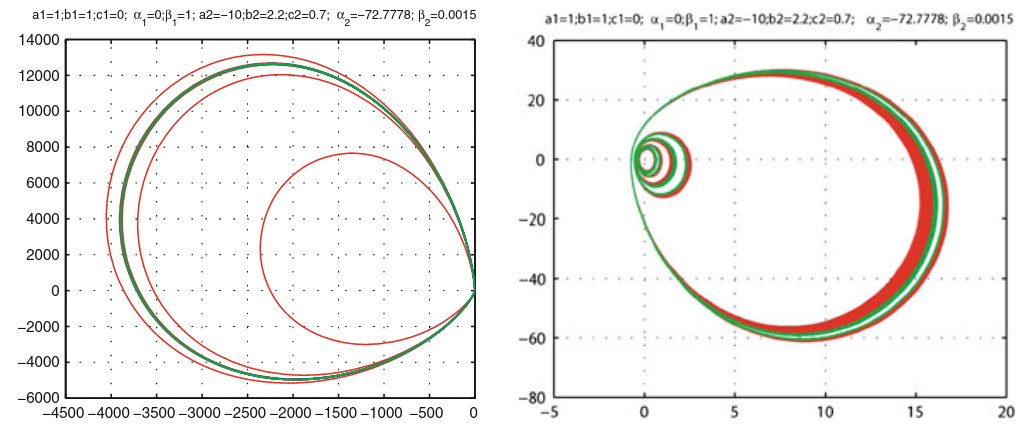
\includegraphics[width=1.0\textwidth]{4cycles}
    \caption{Visualization of four limit cycles in two-dimensional polynomial quadratic system, from Ref.~\cite{kuznetsov_visualization_2013}
    }%
    \label{fig:kuznetsov2}
\end{figure}

\pagebreak
\Cref{fig:kuznetsov_cuda} shows a visualization of the points which a ratio
equal to one with tolerance $10^{-6}$. These correspond exactly with the results
of~\cite{kuznetsov_visualization_2013}. The computation of this data took 250ms
and using a grid of $1024 \times 1024$ trajectories, and a fixed \emph{Runge Kutta}
of third order with a step size of $10^{-3}$. Notice that some points left of $x
= 0$ are not found. Nevertheless, the cycles can be identified easily. Notice that the
4th limit cycle which should be to the left of our plot cannot be found by the program
due to the stiffness of the system on that area. This problem is discussed in more detail
in~\cref{sub:stiffness}. For the rest of the analysis we will only consider
these 3 limit cycles.

\begin{figure}[H]
    \centering
    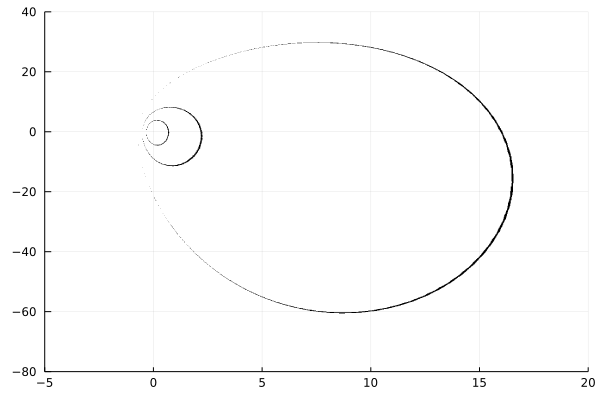
\includegraphics[width=0.8\textwidth]{kutznetsov_cuda}
    \caption{Limit cycles found using our program ($1024^2$ grid)}%
    \label{fig:kuznetsov_cuda}
\end{figure}

Using a bigger grid size of $5000\times5000$, we obtain clearer results but it takes
1200ms. There is not much benefit in this instance since the cycles are clear and
we are searching inside a well delimited plane, but when the search space is greater
it does offer a benefit.

\begin{figure}[H]
    \centering
    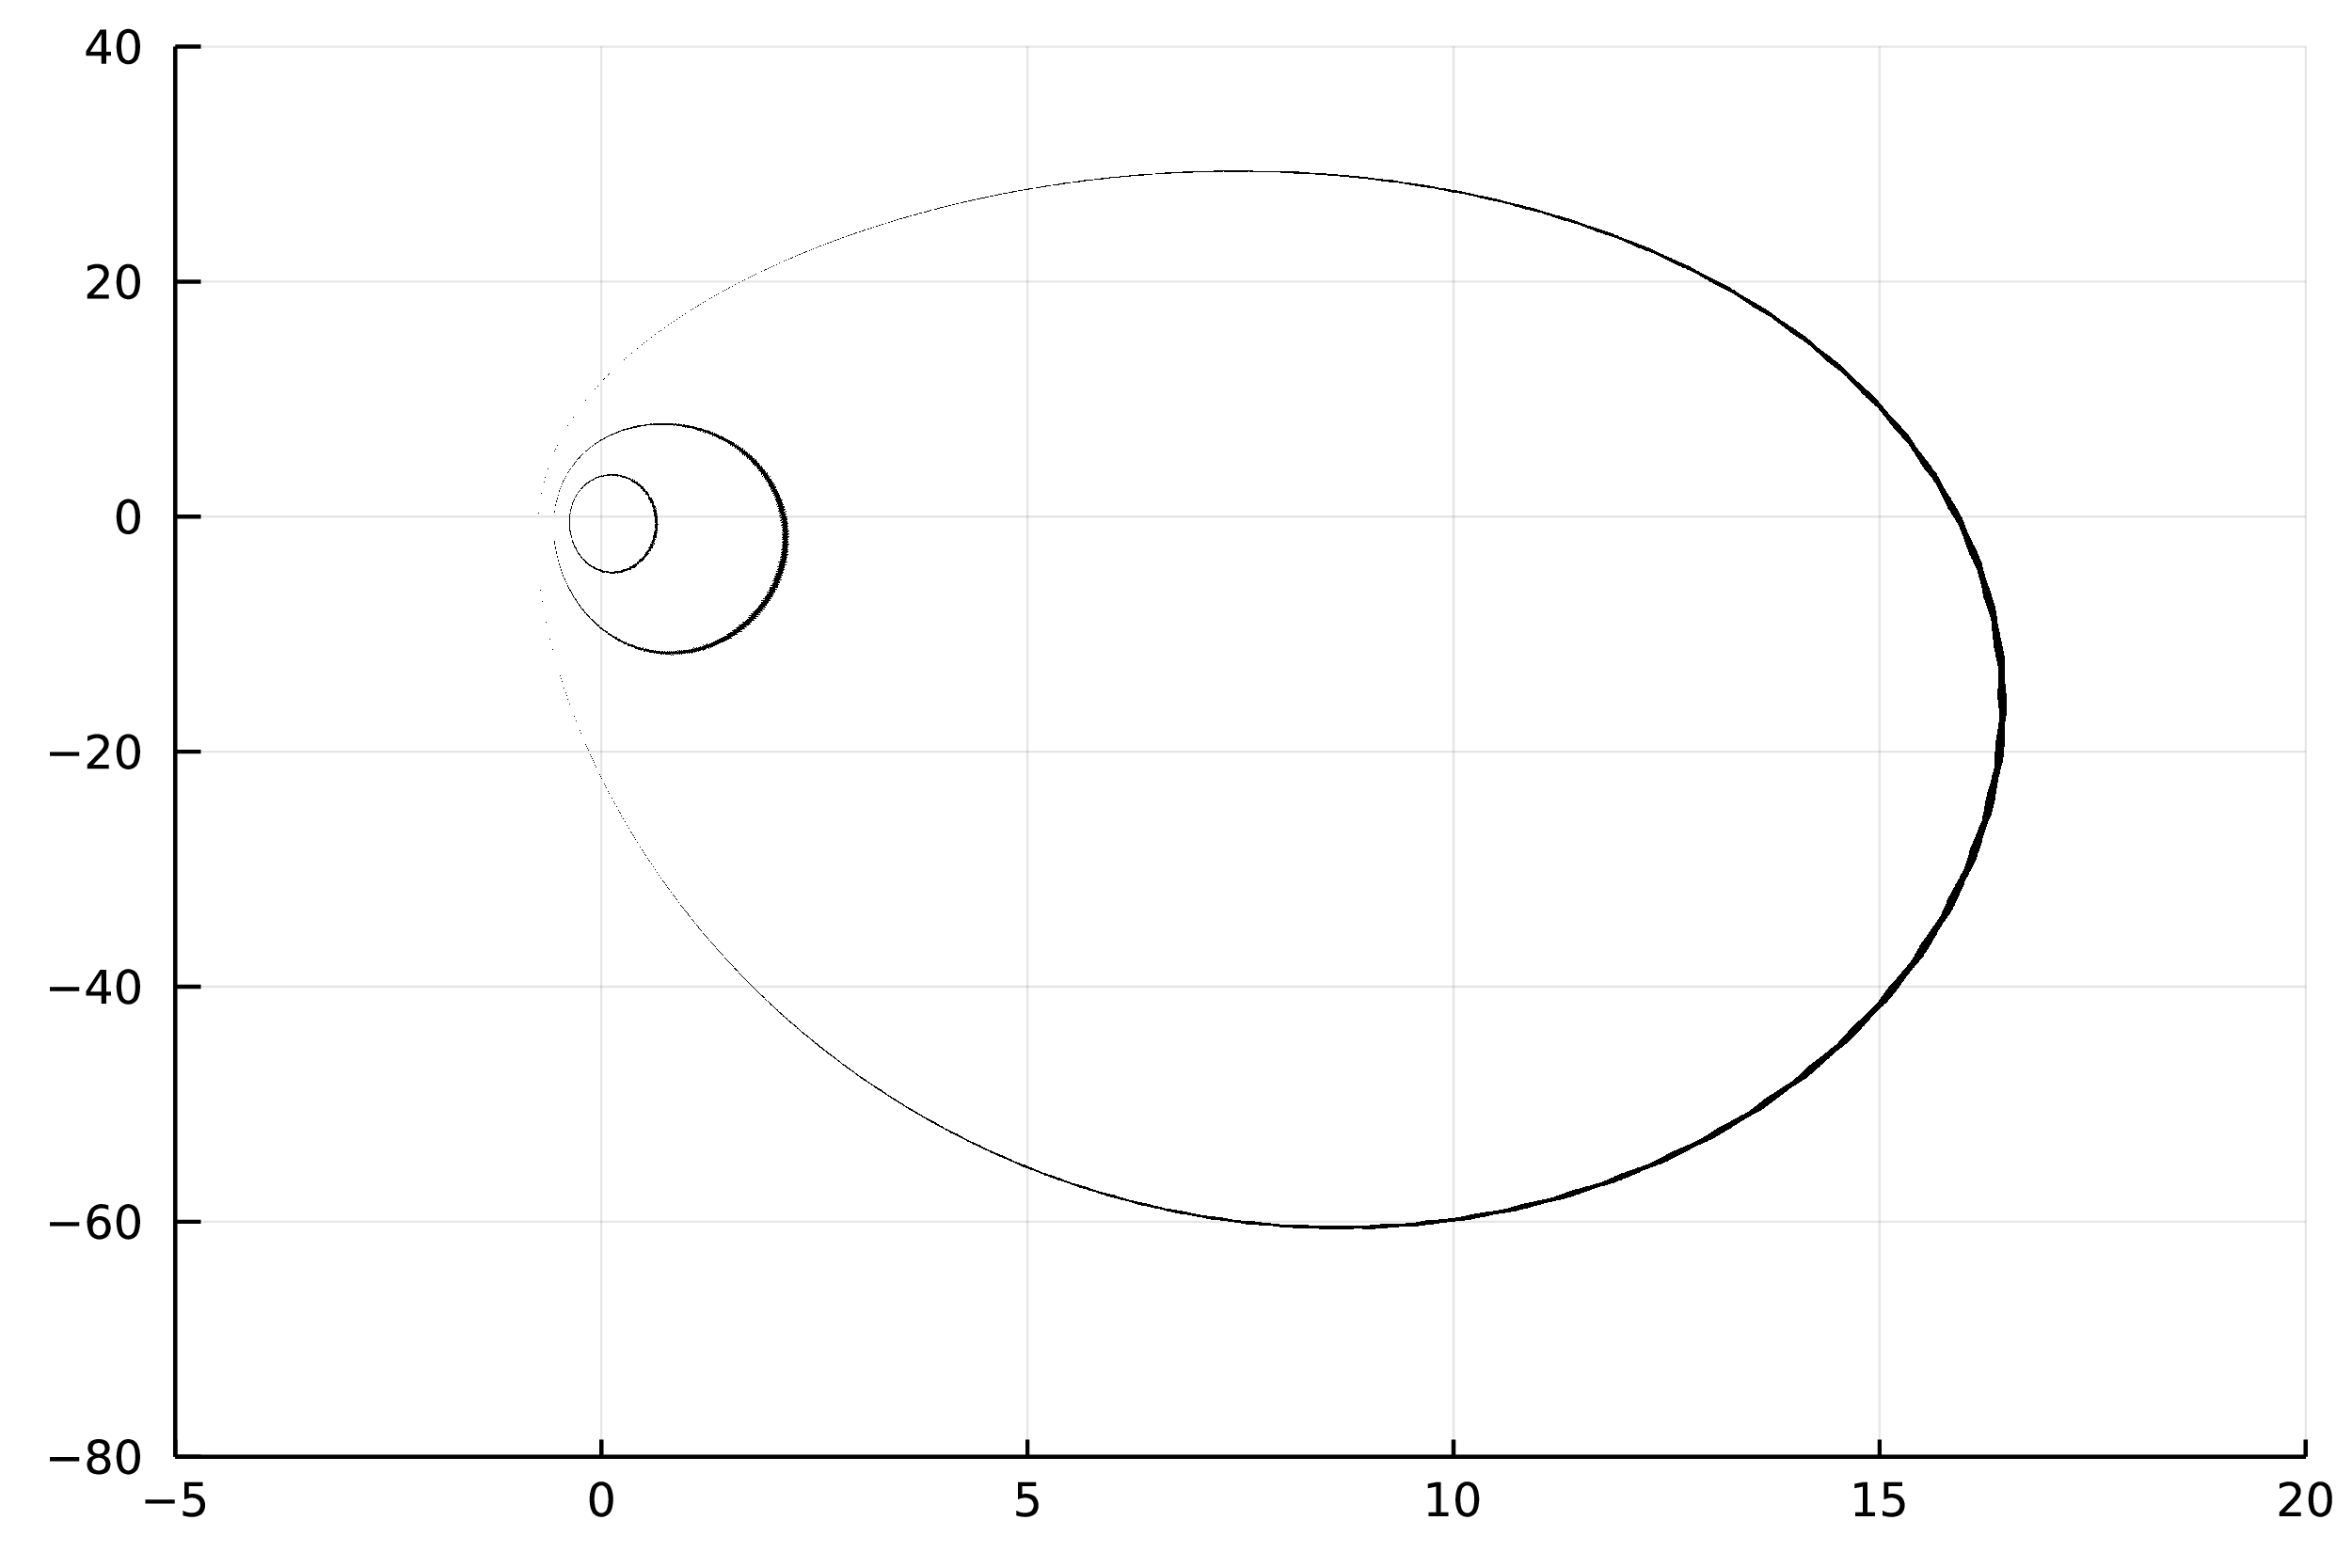
\includegraphics[width=0.8\textwidth]{kutznetsov_cuda_5k}
    \caption{Limit cycles found using our program ($5000^2$ grid)\\
        Black areas correspond to points from which trajectories have
        a rate of 1 (tol $10^{-6}$)
    }%
    \label{fig:kuznetsov_cuda_5k}
\end{figure}

\paragraph{Clustering}

\Cref{fig:histograms} shows the distribution of the 4 different local extrema
values associated with all points with rate of change equal to 1 (with tolerance
$1^{-6}$), we can see that there are 3 clear groups in each one of the local extrema.

If we compute the \emph{K-means} for 3 clusters we obtain the cluster centers shown
in~\cref{tab:clusters}. \Cref{fig:bounding} shows the bounding boxes defined by the
clusters obtained as an overlay over \cref{fig:kuznetsov_cuda}.


\begin{figure}[H]
    \centering
    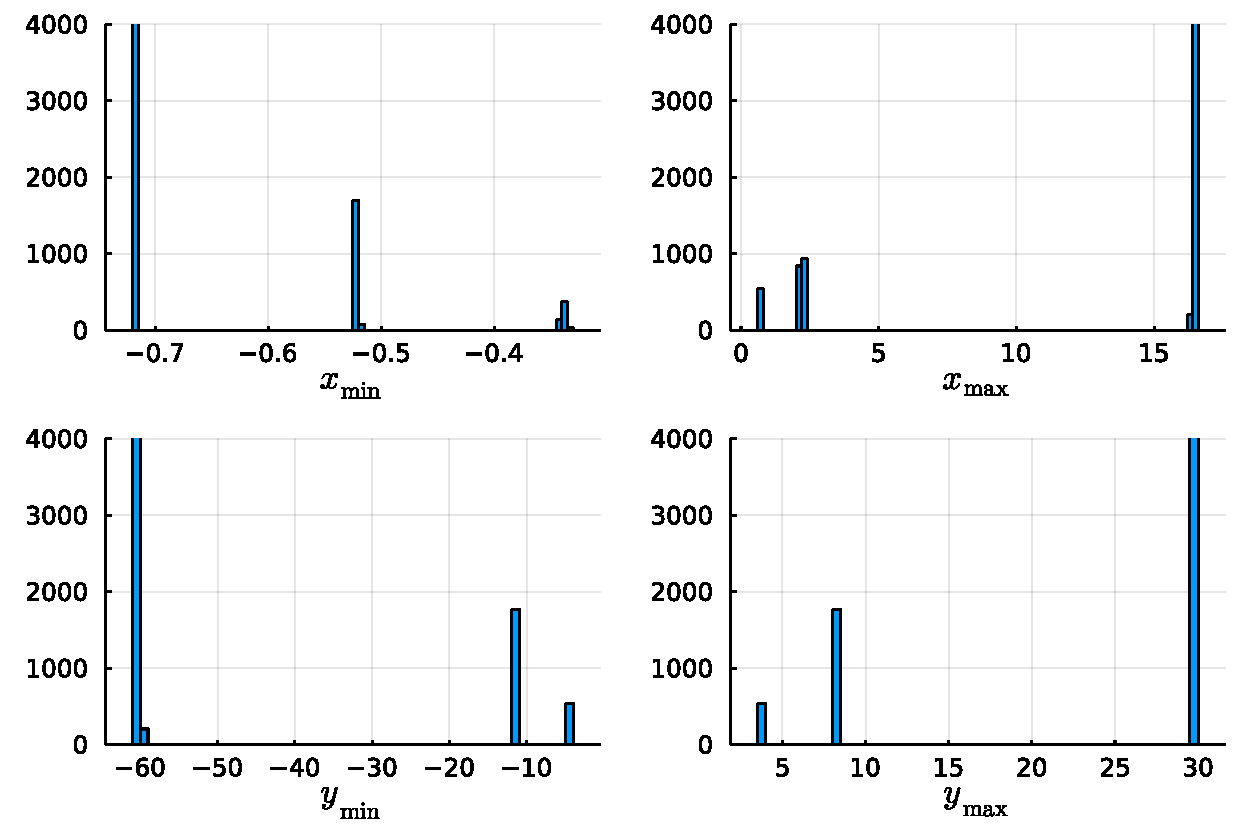
\includegraphics[width=0.8\textwidth]{histograms}
    \caption[Distribution values for local extrema]%
    {Histogram of distribution of values for each local extrema with rate of
        change equal to 1 (tol $1^{-6}$).
    }%
    \label{fig:histograms}
\end{figure}

\begin{table}[H]
    \centering
    \caption{Cluster centers}%
    \label{tab:clusters}
    \begin{tabular}{crrrr}
        \toprule
        Cluster & $x_{\min}$ & $x_{\max}$ & $y_{\min}$ & $y_{\max}$ \\ \midrule
        A & -0.716937 & 16.4835  & -60.2806  & 29.7273 \\
        B & -0.521985 &  2.20031 & -11.3237  &  8.17958 \\
        C & -0.338311 &  0.68522 &  -4.48625 &  3.84119 \\
        \bottomrule
    \end{tabular}
\end{table}

\begin{figure}[H]
    \centering
    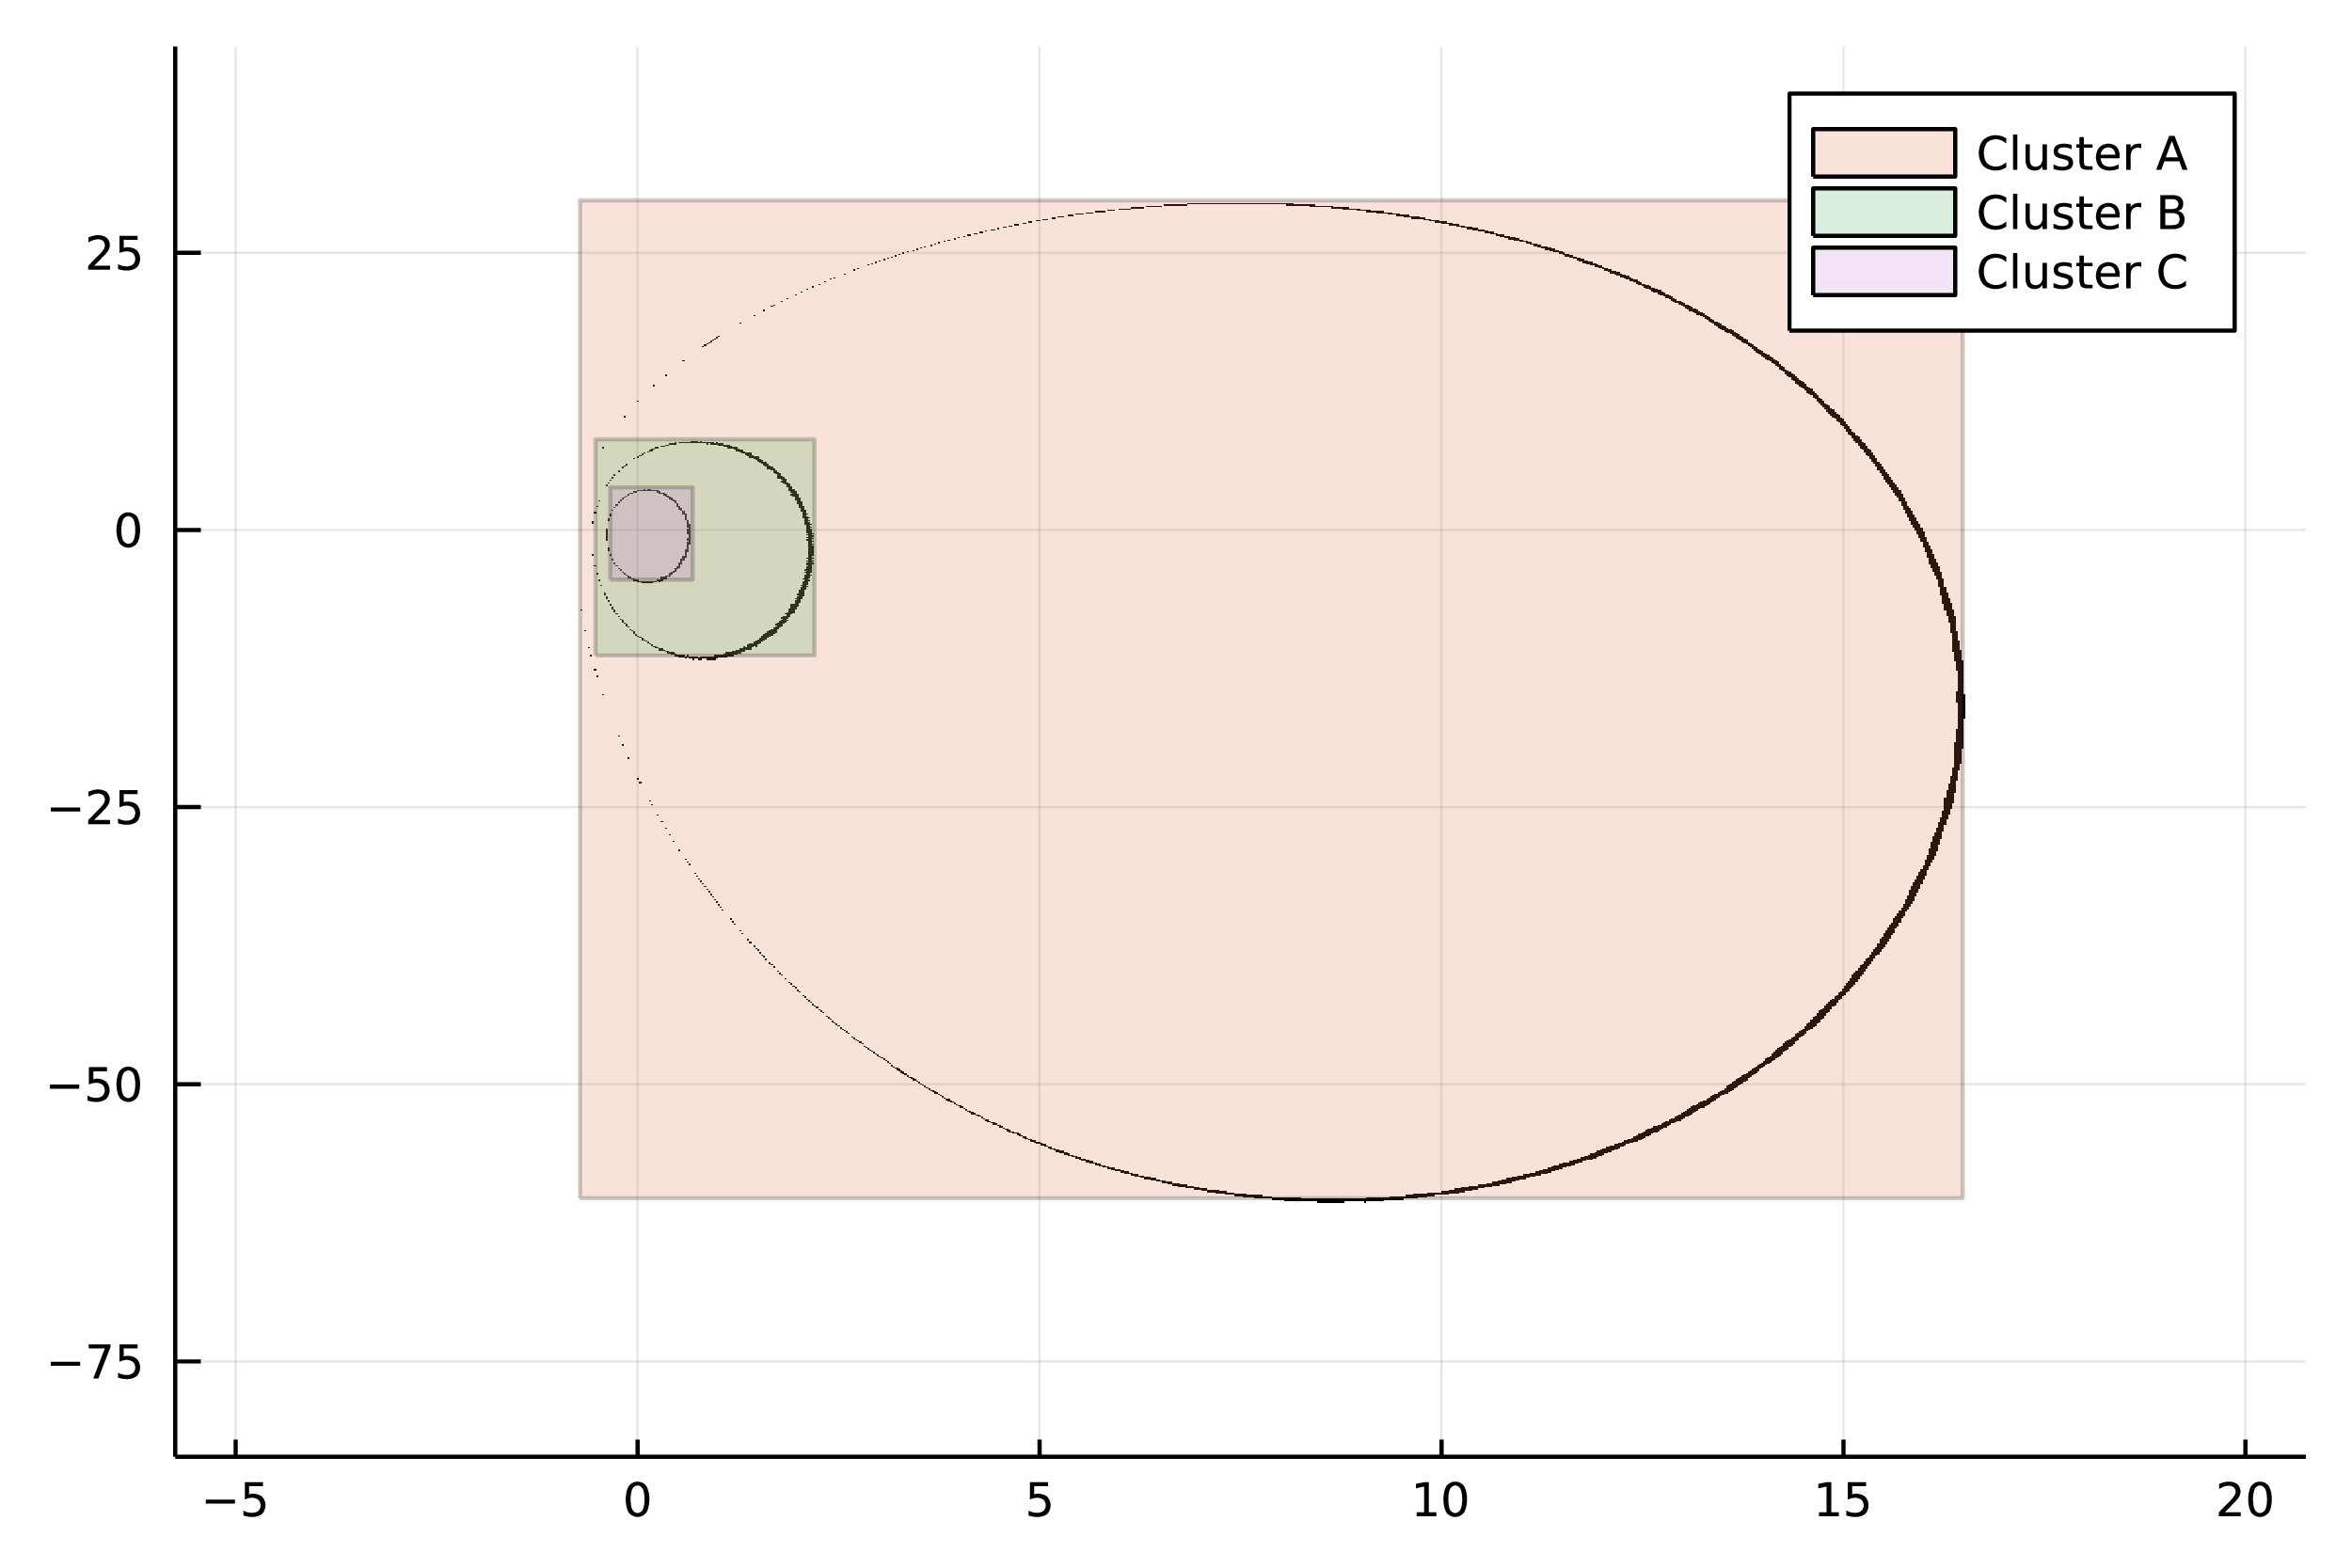
\includegraphics[width=0.8\textwidth]{bounding}
    \caption{Bounding boxes defined by the clusters in \cref{tab:clusters}
        overlaid on top of \cref{fig:kuznetsov_cuda}
    }%
    \label{fig:bounding}
\end{figure}

\pagebreak
\subsection{Applying slight modifications}

\Cref{fig:bounding_a10_1} shows the result of finding limit cycles in the same
system used in the previous examples (\cref{eq:kuznetsov}) but with a slight modification
of parameter $a$ from 10 to 10.1. We can see that the cycles are slightly more similar in size.
Changing to 10.2 only one cycle remains. With $a = 9.9$ there are only two cycles. Other slight
modifications of the other parameters also reduce the number of cycles.

\begin{figure}[H]
    \centering
    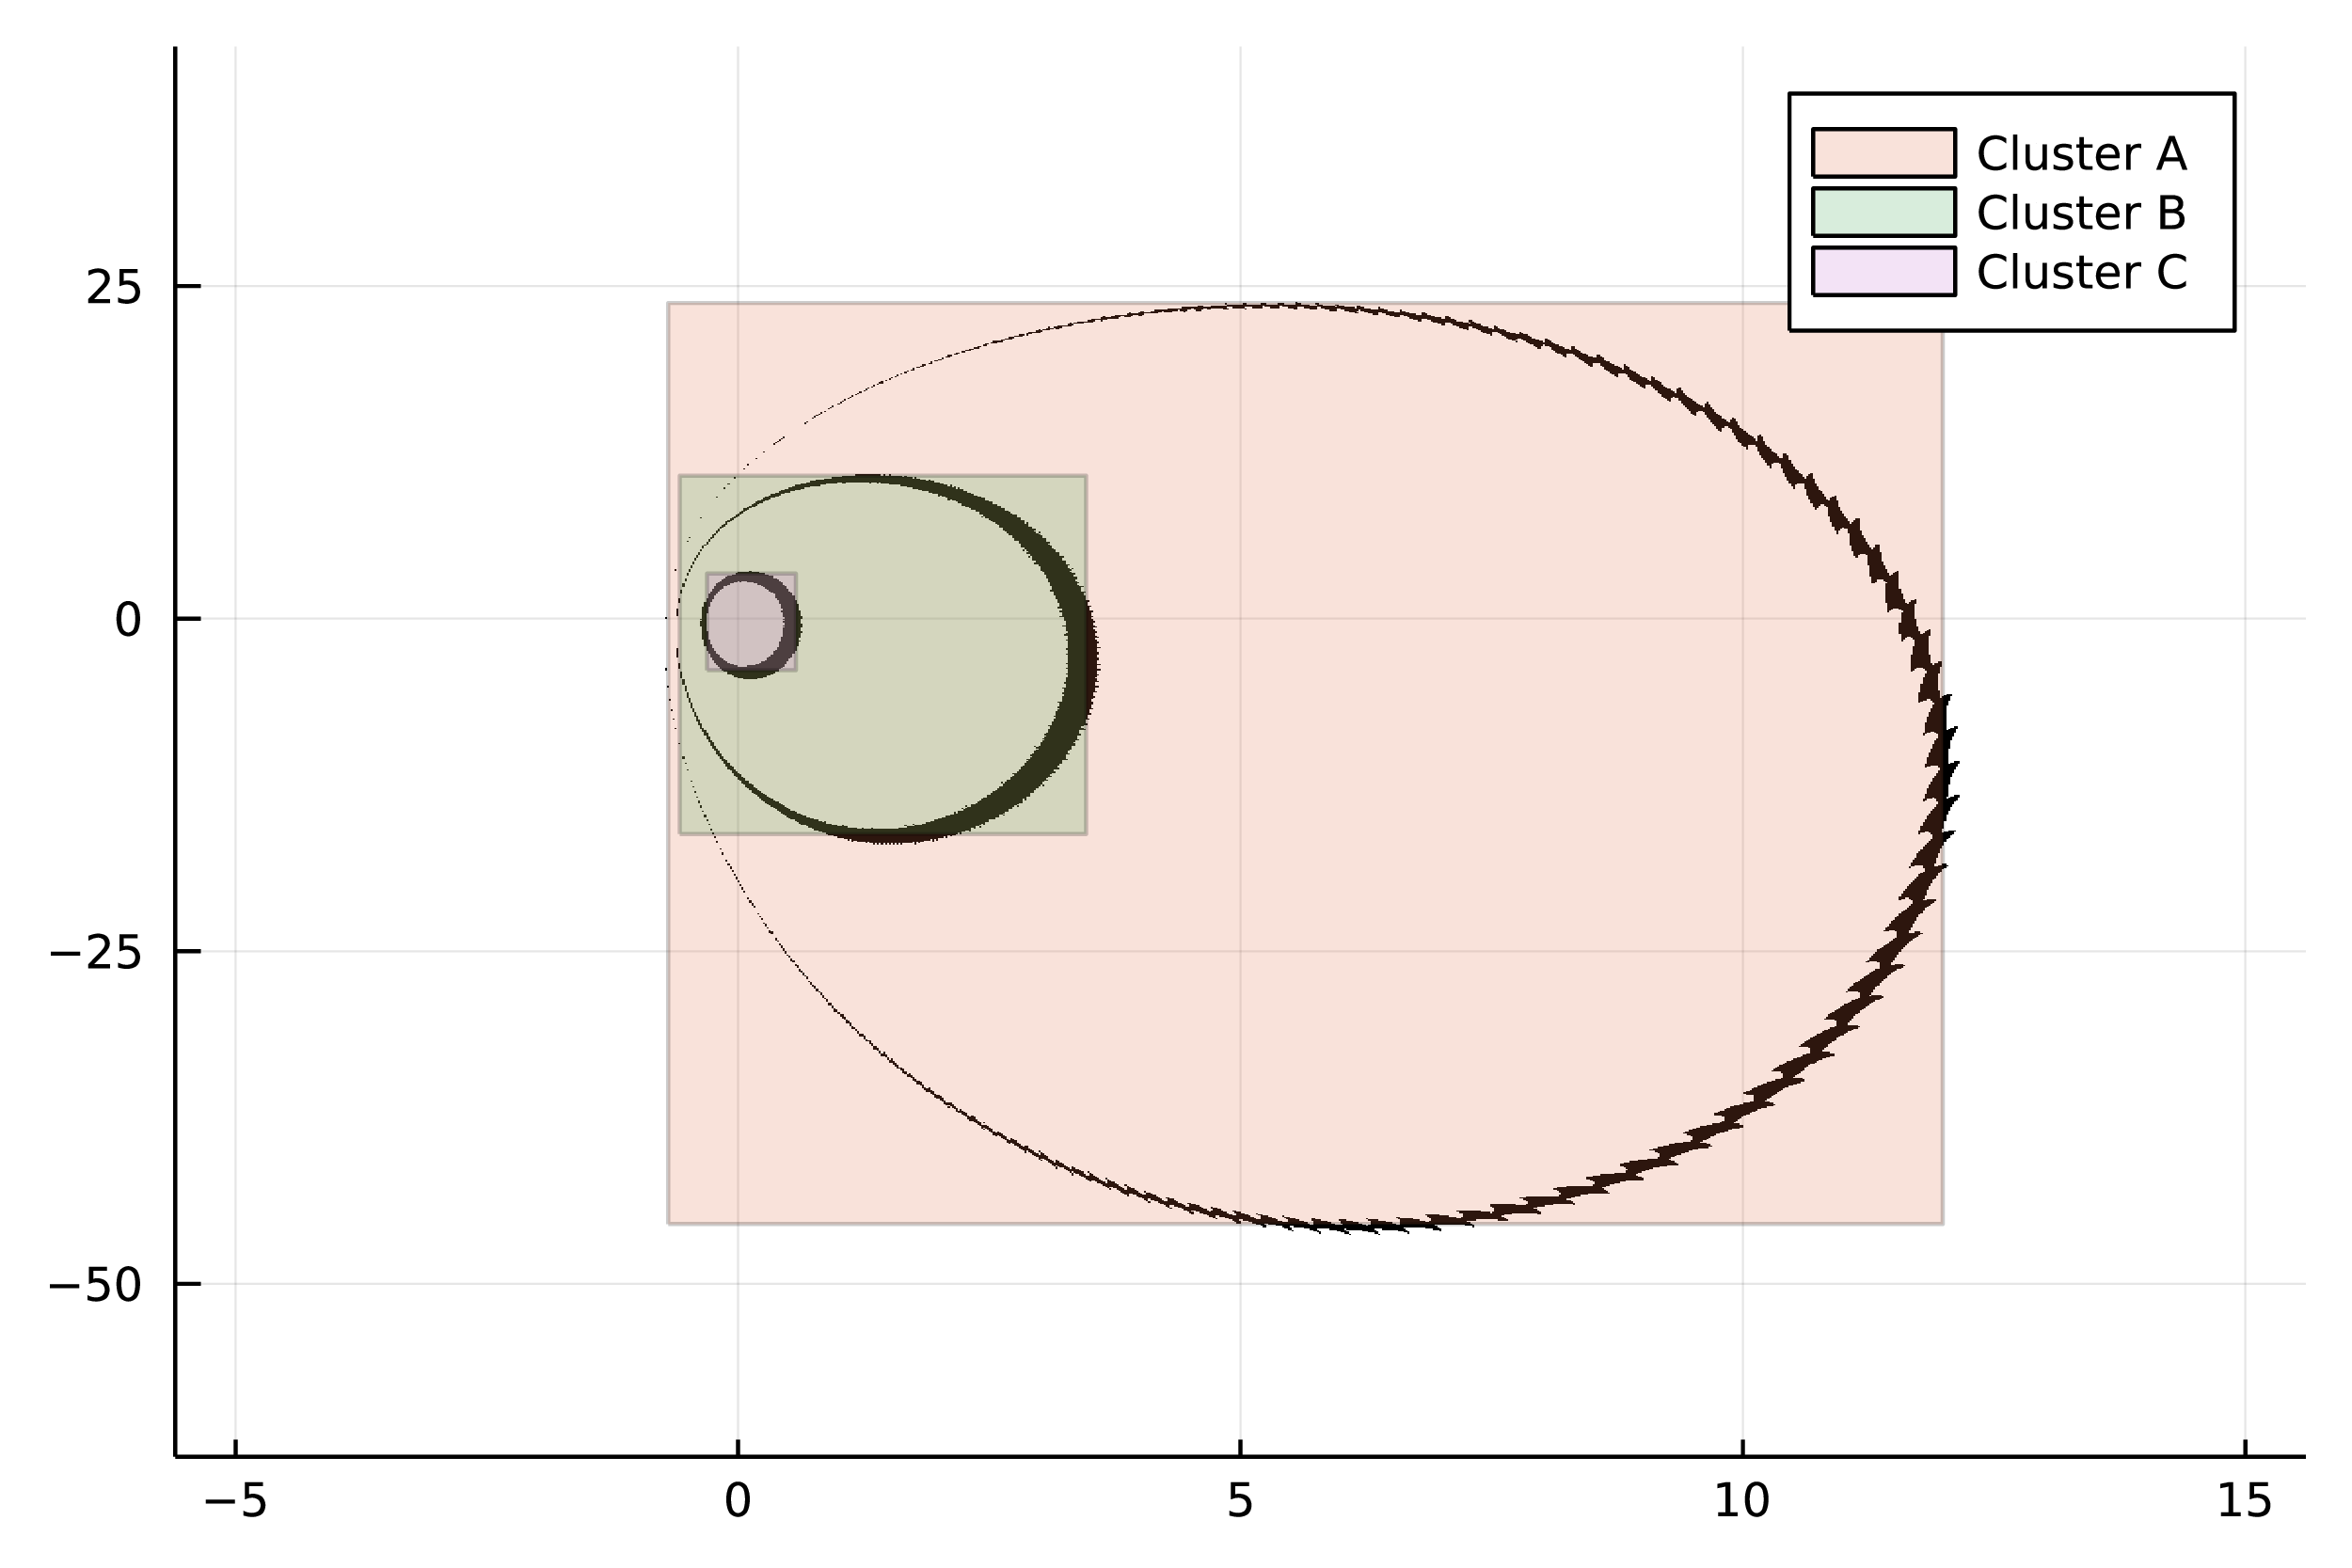
\includegraphics[width=0.8\textwidth]{bounding_a10_1}
    \caption{Limit cycles found on system \cref{eq:kuznetsov} with parameter
        $a$ modified from $10.0 \to 10.1$
    }%
    \label{fig:bounding_a10_1}
\end{figure}

\pagebreak
\subsection{Changing window range}
The previous figures all searched for limit cycles inside the range:
$x \in (-5, 20), y \in (-60, 40)$. In the following section an analysis on the
capacity of the program to find the cycles with different windows will be performed.

\paragraph{Bigger area}

\begin{figure}[H]
    \centering
    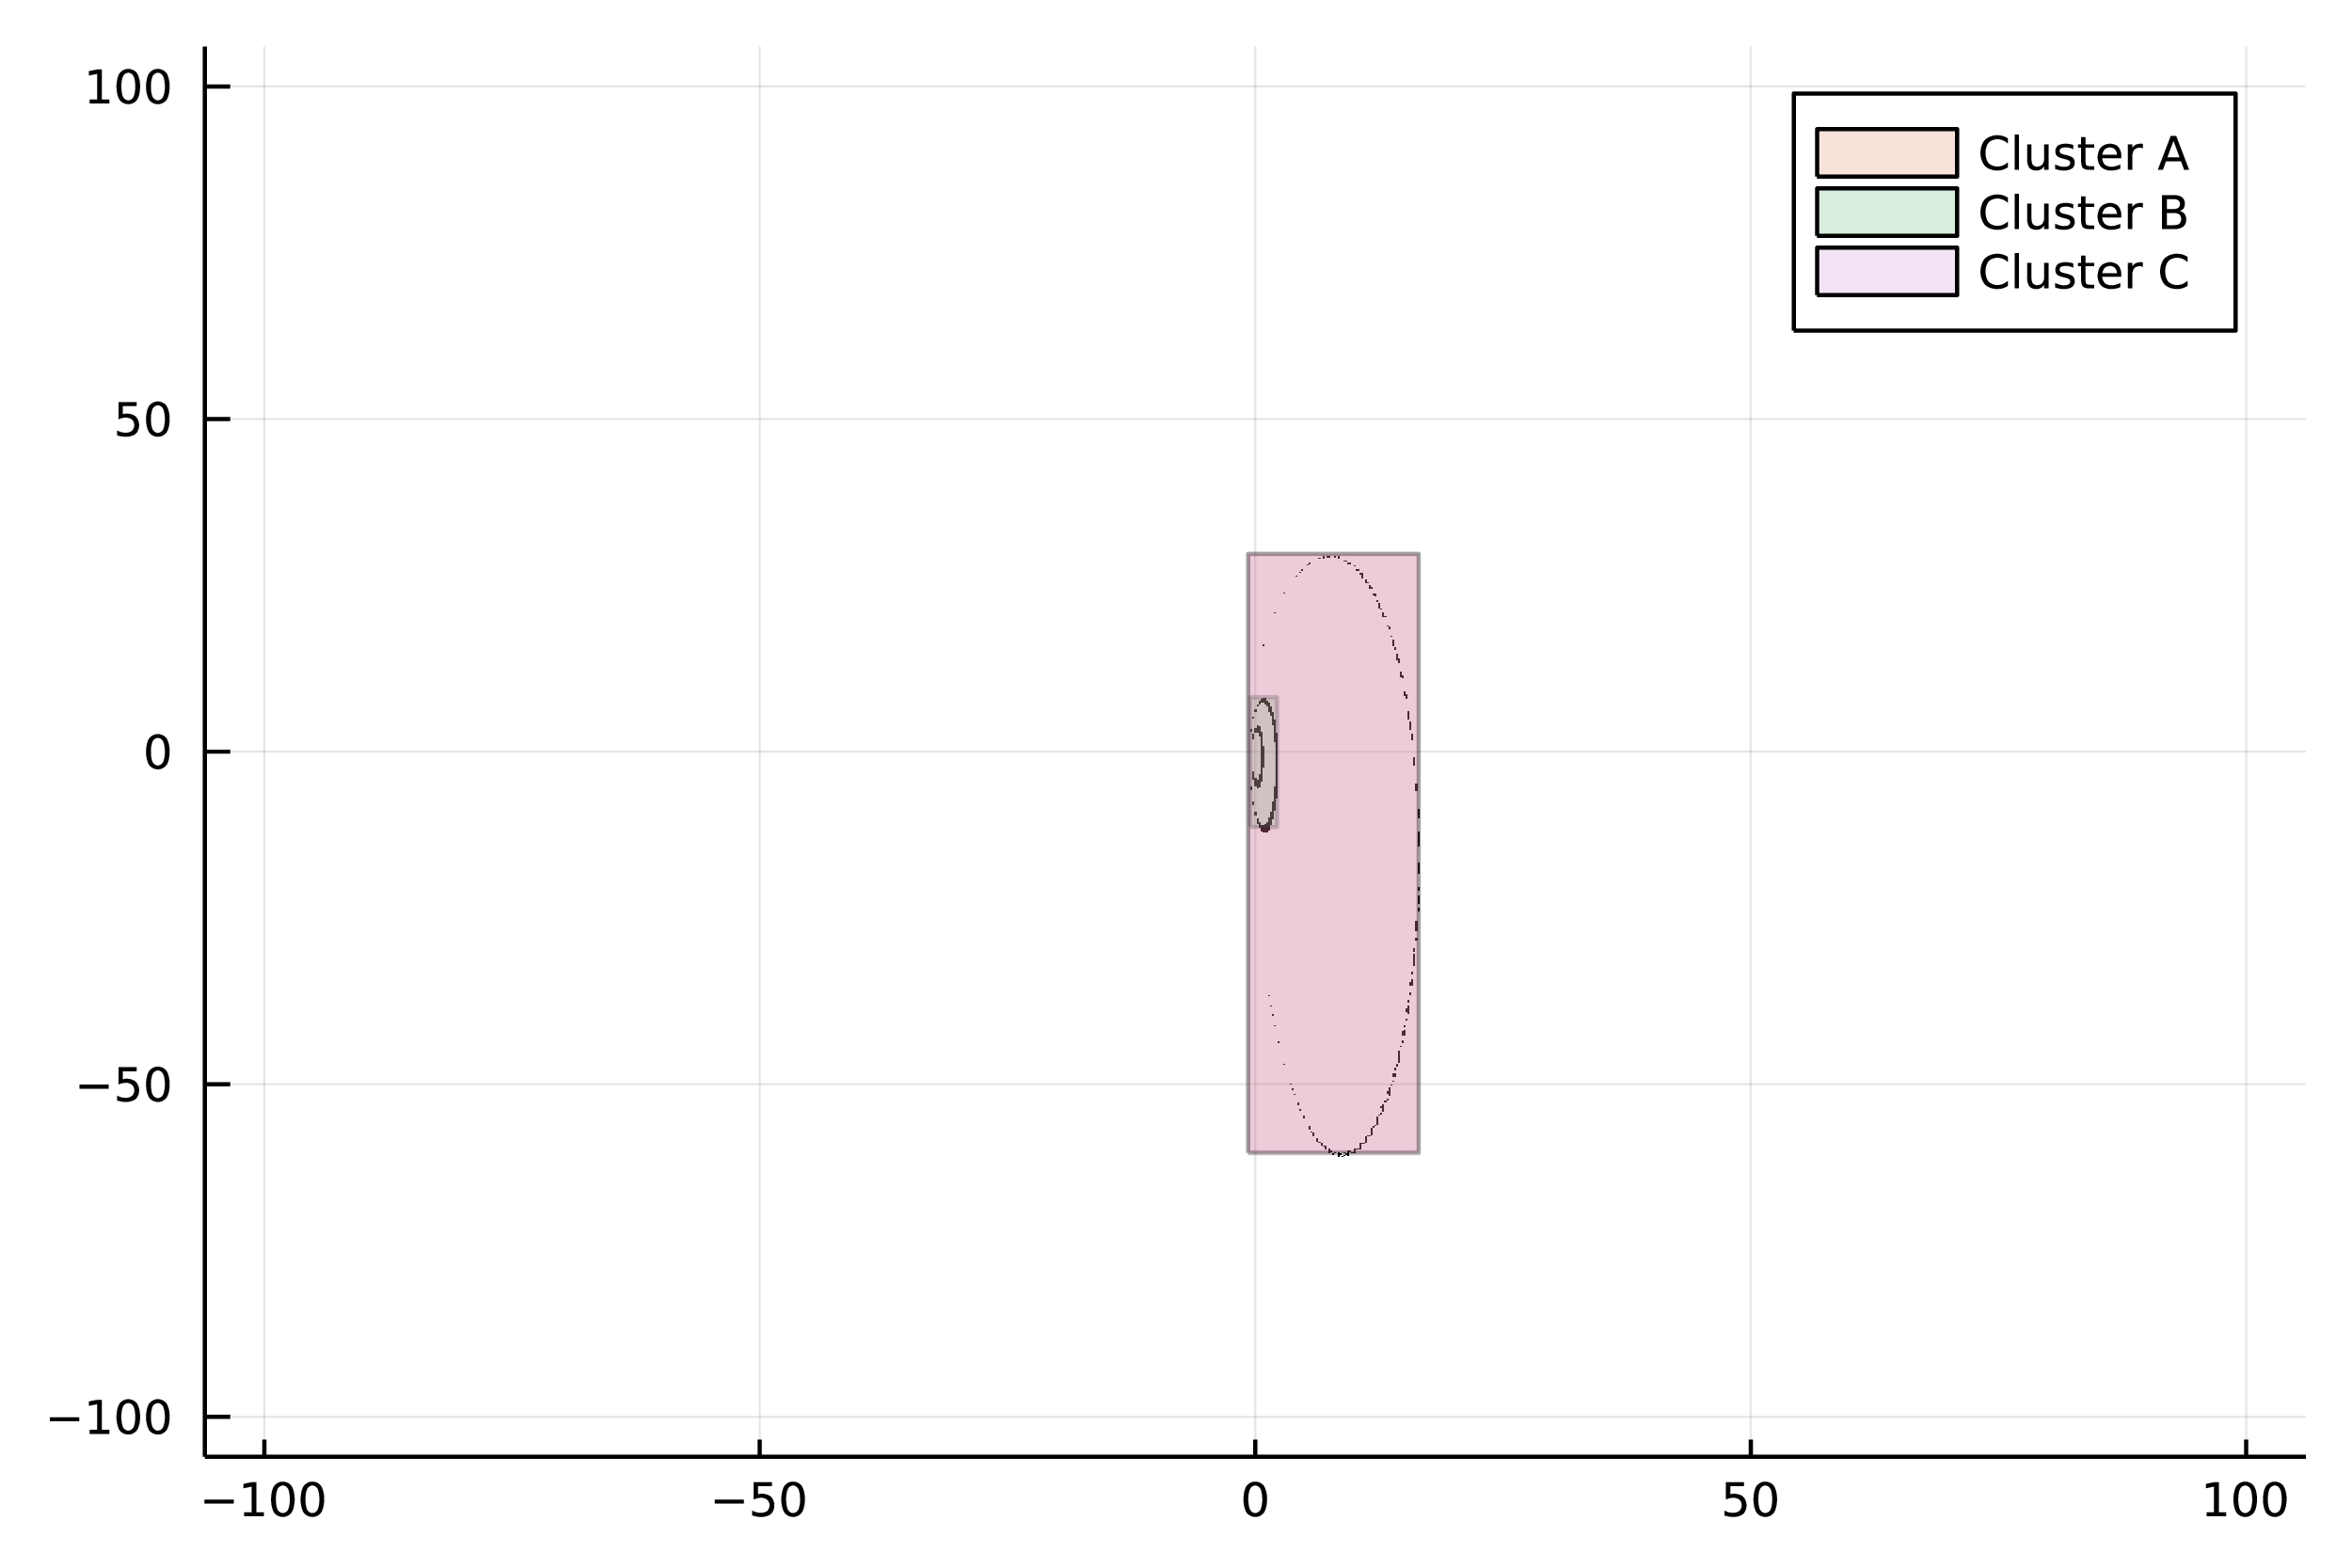
\includegraphics[width=0.8\textwidth]{bounding_100x100}
    \caption{Limit cycles found on system from \cref{eq:kuznetsov} \\
        ($1024 \times 1024$ grid over $x, y \in (-100, 100)$)
    }%
    \label{fig:bounding_100x100}
\end{figure}

As shown in~\cref{fig:bounding_100x100}, with a window of $x,y \in (-100,100)$
we obtain the clusters without problem. Increasing the window further to
$(-1000, 1000)$ does only find the two bigger limit cycles. A possible optimization
could be to make two pases, one to find the bigger limit cycles and a second one using
as a window the bounding box of the limits found.

\pagebreak
\paragraph{Partial occlusion}

The algorithm should be robust to partial occlusion of the cycle, meaning that
even if part of the cycle is outside the window it should still be detected.
In~\cref{fig:bounding_occ} we show an image of the results applied with a window
of $x \in (0, 5), y \in (0, 20)$ (Shown in gray). The clusters are equivalent as
the ones in the previous examples. Note that the line of the biggest cluster is very thin
since there are not many points. As long as the window contains enough part of the trajectory of
a limit cycle\footnote{And the trajectory is not stiff (see \cref{sub:stiffness})} with
enough resolution, the cycles can be identified.

\begin{figure}[H]
    \centering
    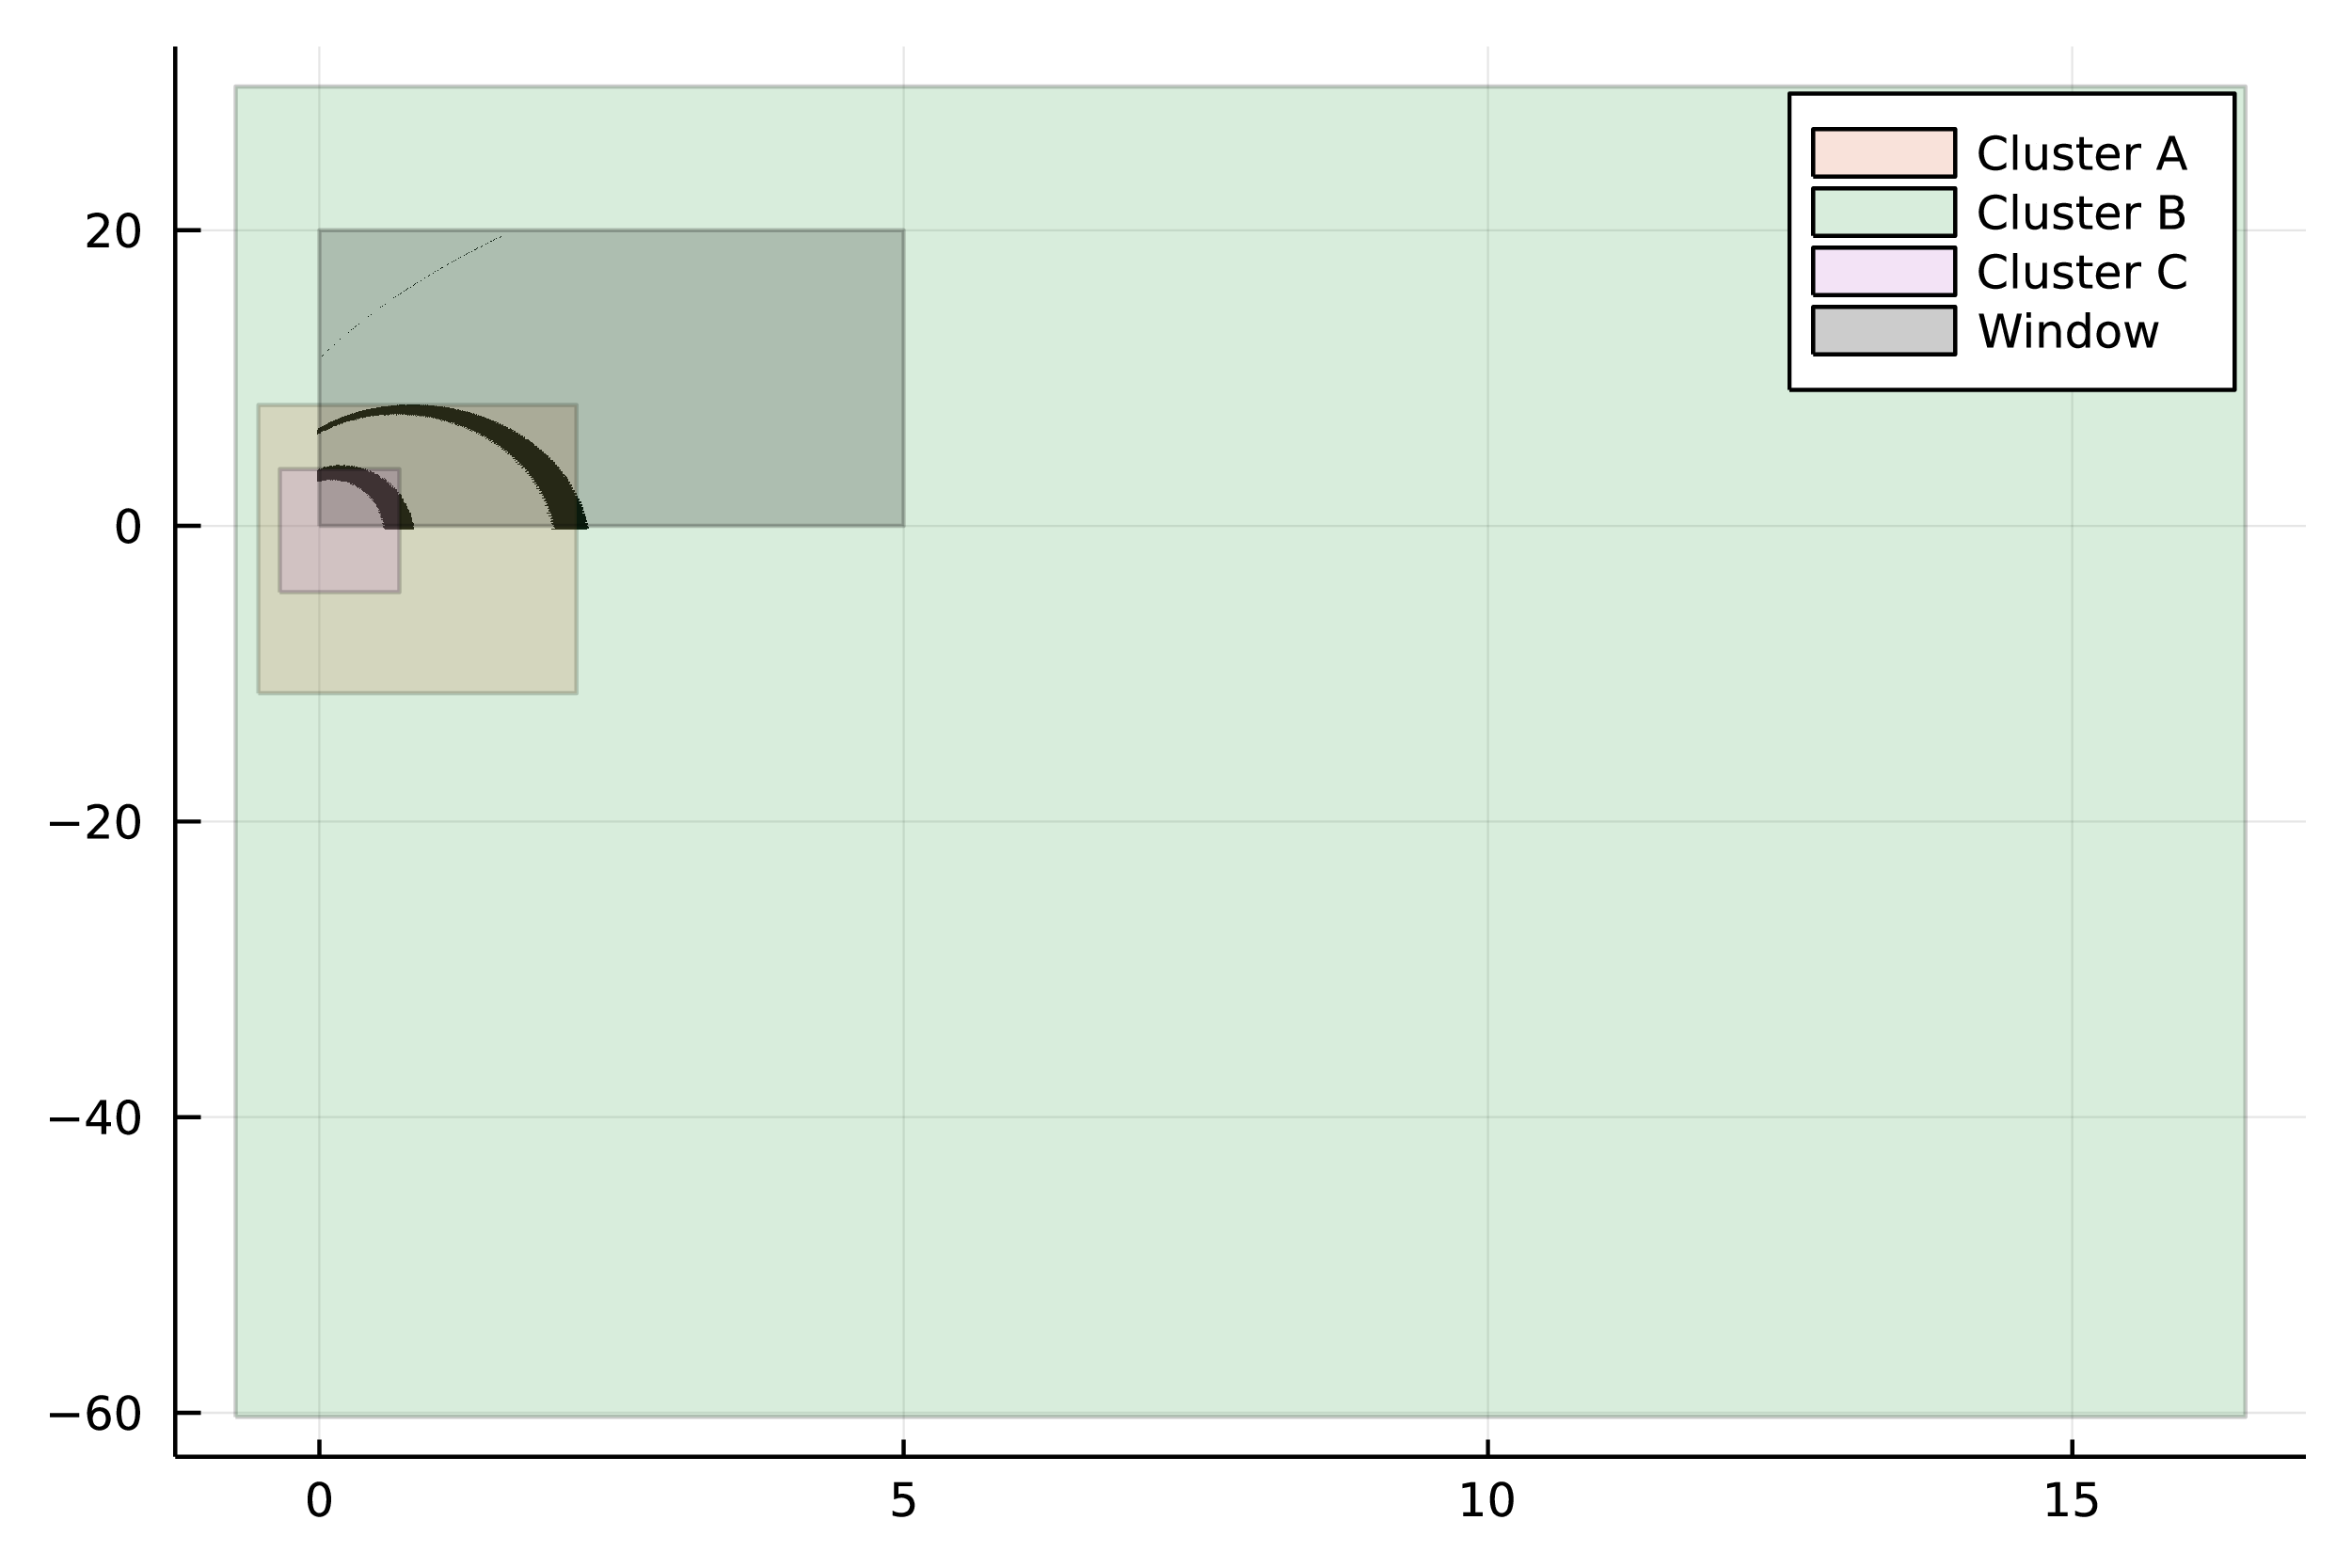
\includegraphics[width=0.8\textwidth]{bounding_occlusion}
    \caption{Limit cycles found on system from \cref{eq:kuznetsov} \\
        ($1024 \times 1024$ grid over $x \in (0, 5), y \in (0, 20)$)
    }%
    \label{fig:bounding_occ}
\end{figure}

\pagebreak
\paragraph{Compactified plane}

Since the plane in $\mathcal{R}^2$ is infinite, in order to visualize limit cycles without
restricting portions of the plan a compactification should be performed.
In \cref{sec:compact-stiff} there is a more in depth explanation of how this can be done. In
our case the compactificaction is rather simple and just involves calculating the tangent,
reducing the plane from $(-\infty, \infty)$  to $(-\pi/2, \pi/2)$. This compactification is
not ideal since it deforms the plane a lot, but allows to perform a more wide search of cycles.
Although it does not help if they are big since they get \emph{squished} on the borders. The
result of applying the tangent compactification and running the program is shown
in~\cref{fig:bounding_compact}. The biggest cycle is almost non visible despite the fact that
it is not particularly big ($y_{\min} \approx -60, y_{\max} \approx 30$).

\begin{figure}[H]
    \centering
    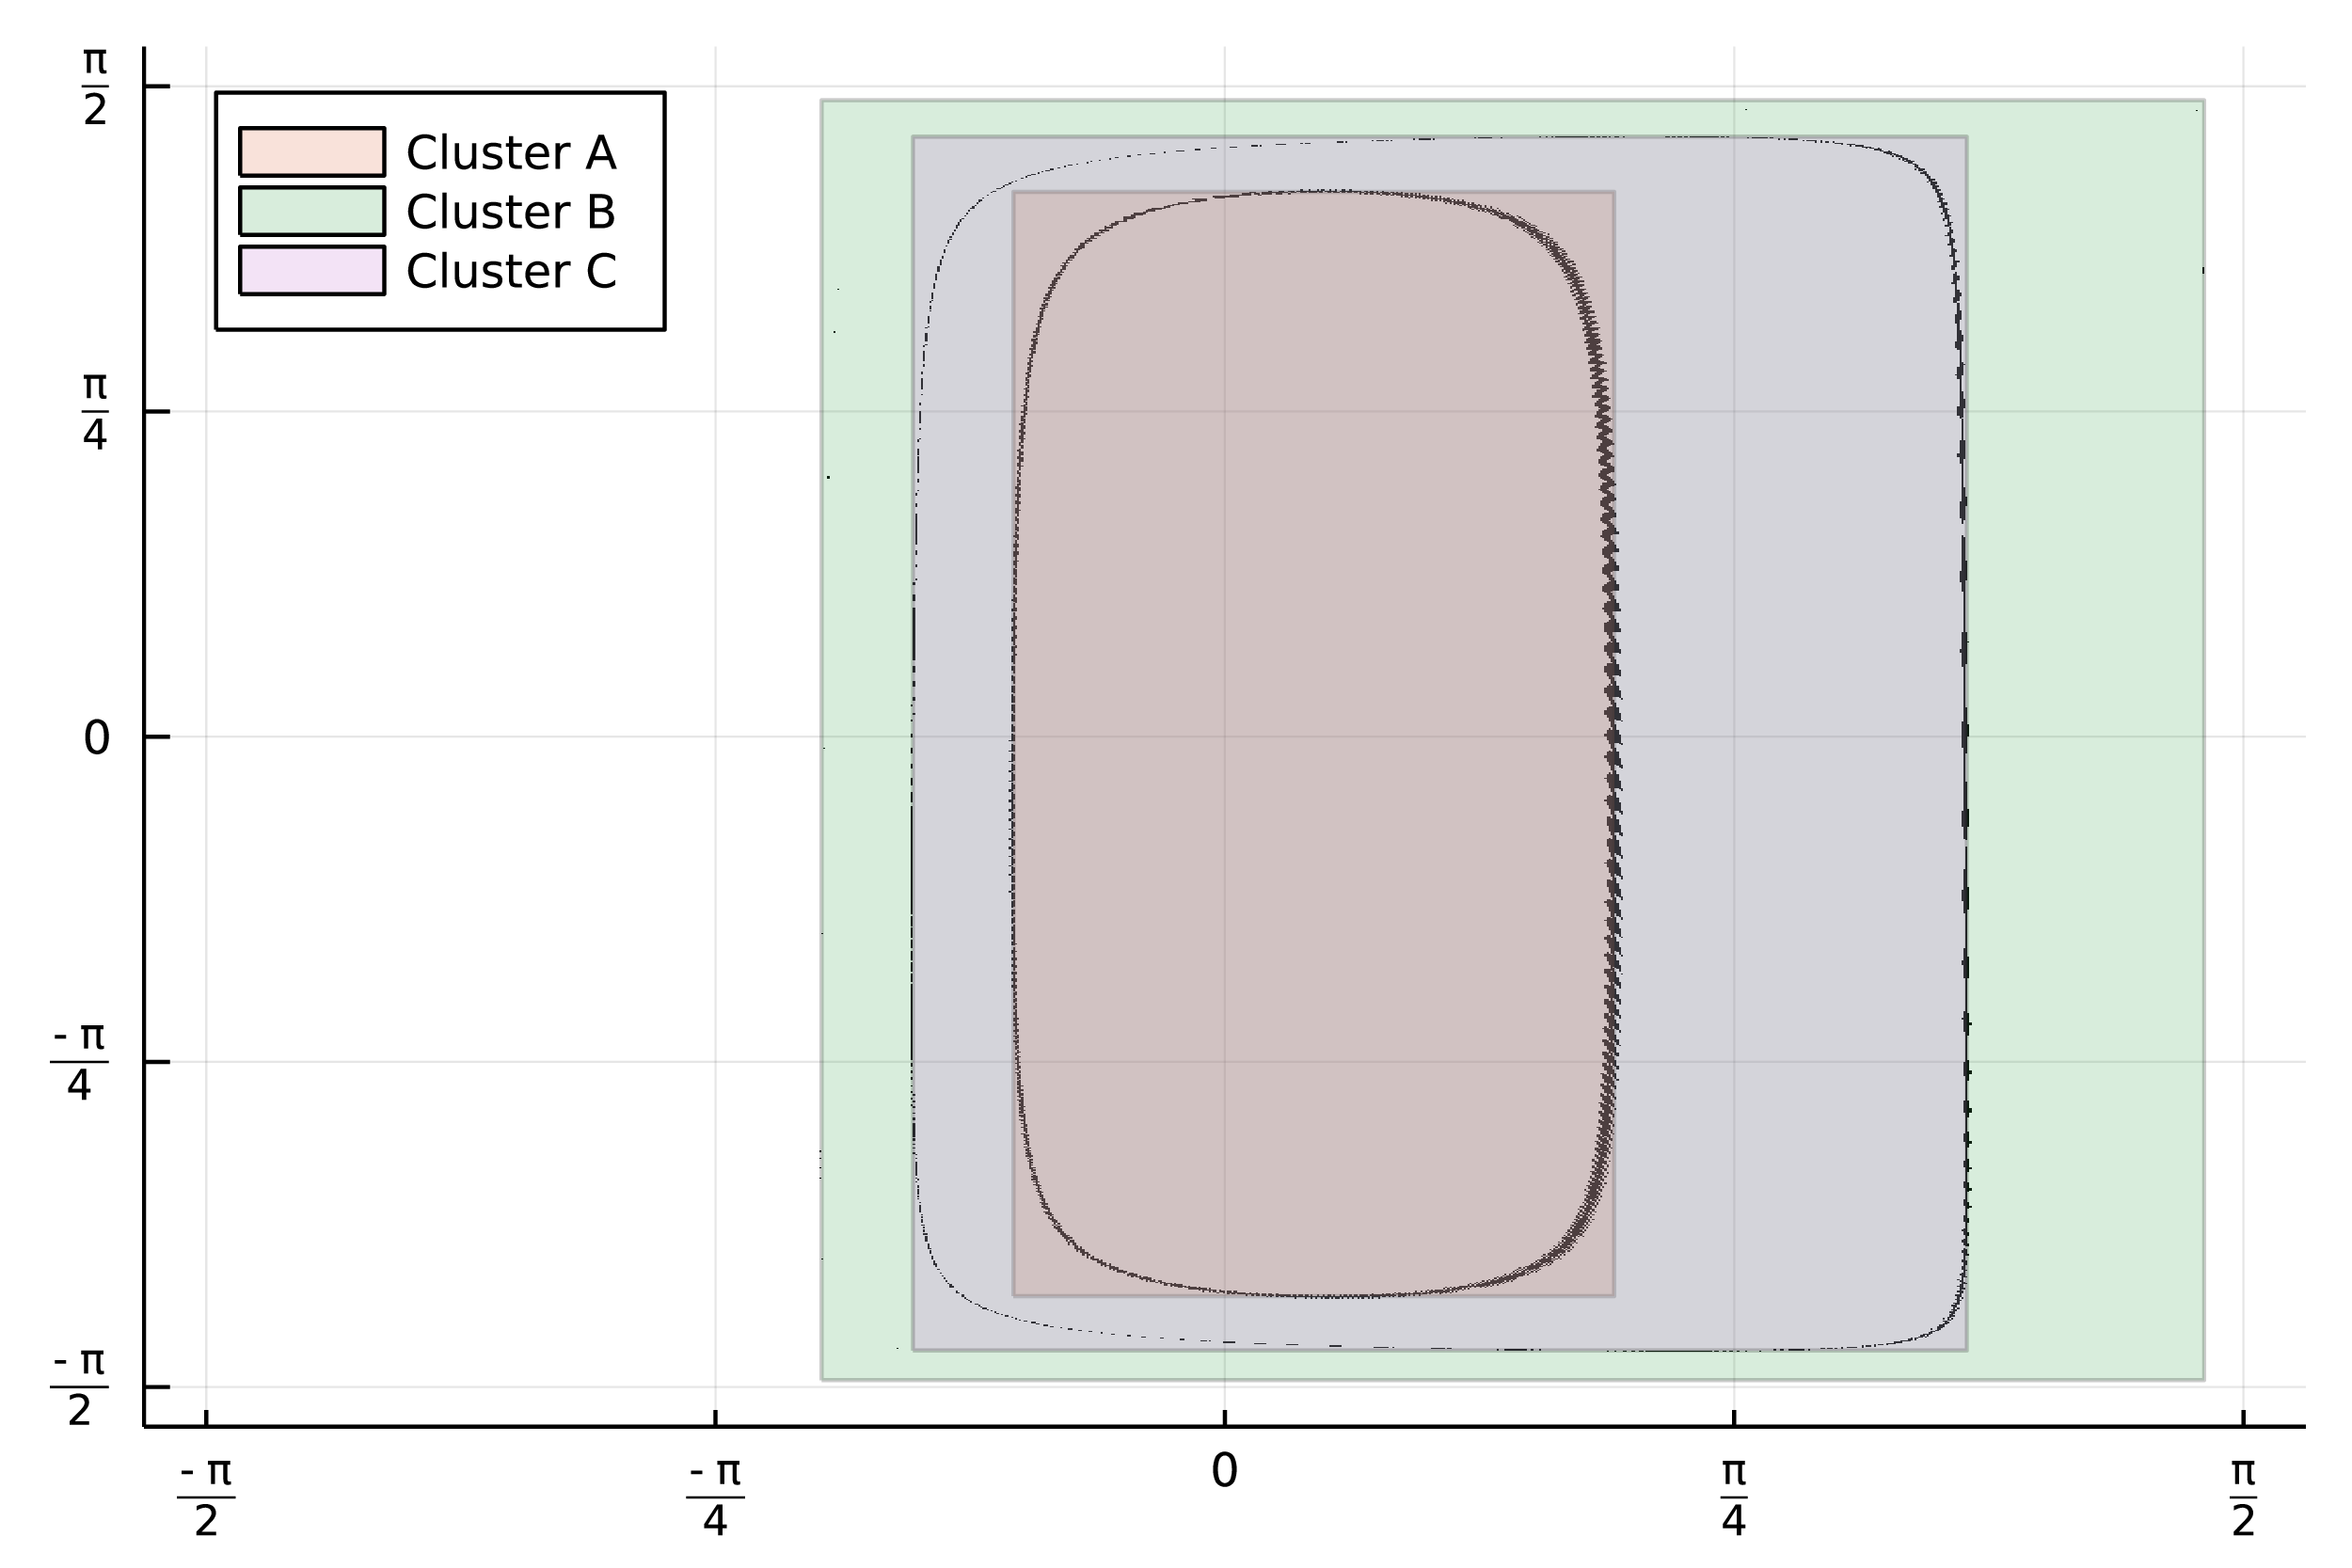
\includegraphics[width=0.8\textwidth]{bounding_compact}
    \caption{Limit cycles found on system from \cref{eq:kuznetsov} \\
        ($1024 \times 1024$ grid over compactified plane)
    }%
    \label{fig:bounding_compact}
\end{figure}

    %! TEX root = **/010-main.tex
% vim: spell spelllang=en:

\section{Performance analysis}


In this section we analyze the runtime performance of the CUDA part of
the program compared to the same implementation sequentially in C. All
these measures are done using the same kernel that computes the ratio
of local extrema for each point. The grid size refers to the number of
points in the grid: a grid of size $2^14$ corresponds to a
grid with $2^7$ points in both $x$ and $y$ ($2^7 \times 2^7$). For each of these
$2^14$ points a trajectory is computed. In these benchmarks the trajectories were
performed using the \emph{Runge Kutta} of order 3 with a step size of 0.0001 and
10000 steps.


\begin{figure}[H]
    \centering
    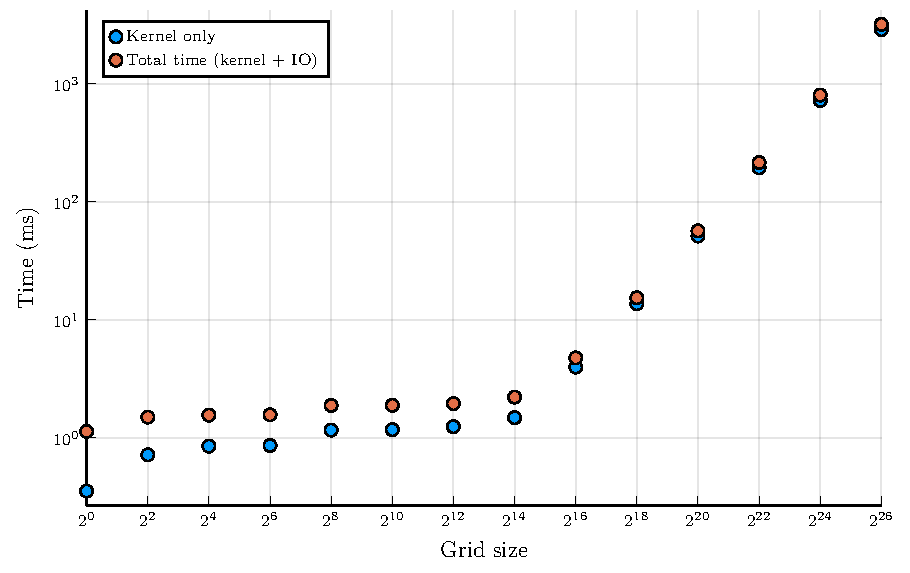
\includegraphics[width=1.0\textwidth]{e_time_kernel}
    \caption{Execution time of CUDA version with separate kernel time
    }%
    \label{fig:time_overhead}
\end{figure}

\Cref{fig:time_overhead} shows the execution time of the CUDA version with a
separate measure for the time spent in the kernel (the actual calculation). Total
time is the time spent in the kernel plus the additional time for input/output
operations and CUDA synchronization directives. For grid sizes of 1 and 2, most of the
time is spent outside the kernel. We can observe that the time is roughly the same
from grid sizes $1$ to $2^14 (16384)$ but after that there is a notable increase.
This is due to the fact the GPU used has 10240 CUDA cores so
we are using all cores and reaching the parallelization limit of the device.

If we now add the execution time of the \emph{C} sequential implementation of the
program we obtain~\cref{fig:time_cuda}. The CUDA version outperforms the sequential
version for grid resolutions as low as $4\times4$. This is due to the nature of the
computation which has very little overhead on copying operations between the GPU and
CPU, allowing for really notable performance gains. The quadratic fit on the sequential time
shows how it increases quadratically with the grid resolution.

\begin{figure}[H]
    \centering
    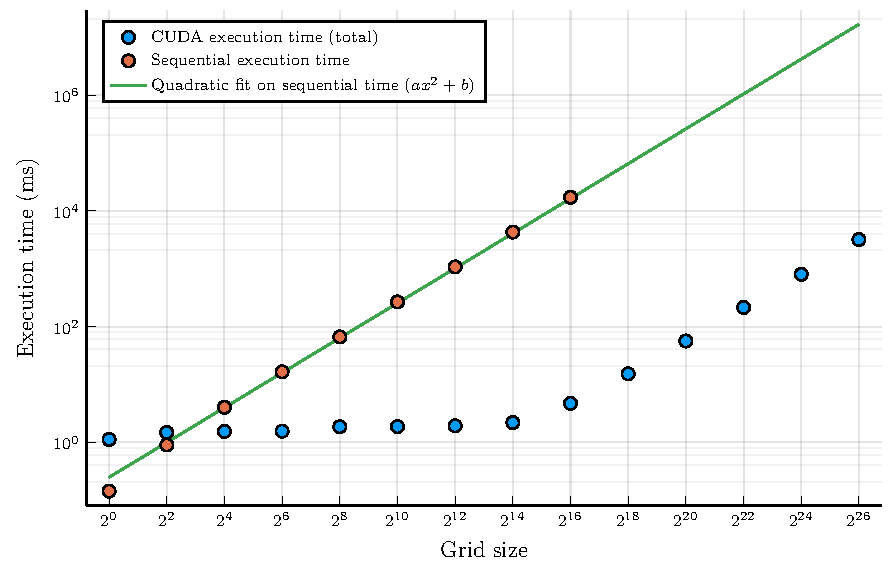
\includegraphics[width=1.0\textwidth]{e_time_all}
    \caption{Execution time of CUDA version vs. Sequential}%
    \label{fig:time_cuda}
\end{figure}

% {\bf define speedup ???}

By computing the ratio between the execution time of the sequential version and the CUDA
version, we obtain the \emph{Speedup}, which indicates how much faster the CUDA computation is
compared to the sequential version. As stated before the GPU used has 10240 cores so the
theoretical maximum speedup is 10240. Obviously such speedup is not feasible, both due to the
fact that a CPU core runs faster than a CUDA core and that there are additional operations
of communication between CPU and GPU that increase the execution time.
The dependence of the speedup on the number of trajectories is shown in \cref{fig:speedup}.

\begin{figure}[H]
    \centering
    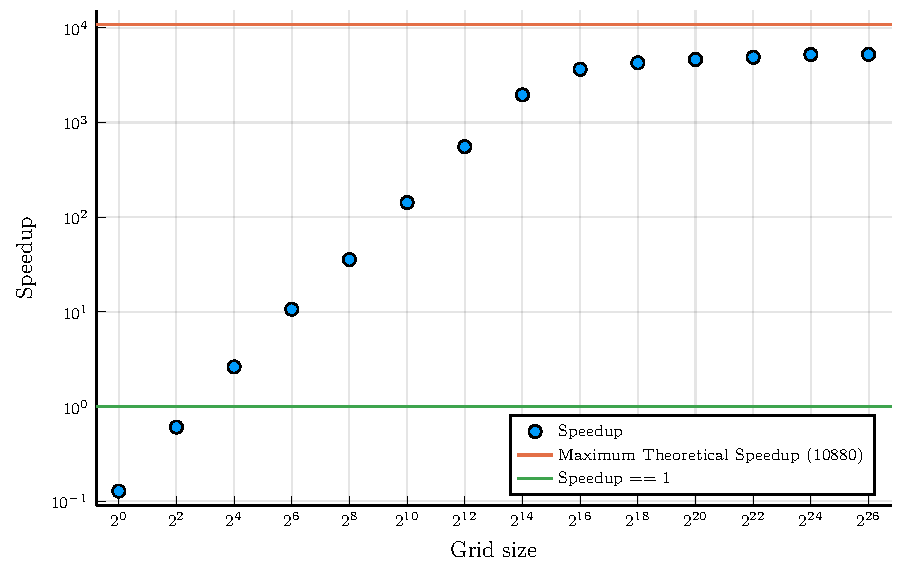
\includegraphics[width=1.0\textwidth]{speedup}
    \caption{Speedup of CUDA version vs. Sequential}%
    \label{fig:speedup}
\end{figure}

The overhead for starting CUDA processes make the GPU code slower for
calculation of small number of trajectories. For $\approx 2^4 = 16$ trajectories
the parallel and the serial codes require a similar execution time. The parallel
code runs faster (speedup larger than one) for larger number of trajectories.
The theoretical maximum for speedup is limited by the number of cores in GPU
(10240 in the present case) while here we observe $5239$ at maximum. There is
still an order of magnitude from the maximum achievable speedup which gives room
for improvement. Specially if we use additional GPUs. For reference, the
computation of $2^{26} \approx 6\times 10^7$ trajectories took 3.202s on the GPU
while the sequential version of the program would take approximately 4 hours and
40 minutes.  This massive computation of $2^{26}$ trajectories requires around 7
Gb of GPU memory if using and polynomial interpolation (although there is only
550Mb of data to needed for the final result). Given that the GPU has 12 Gb of
memory, higher resolutions cannot be performed with this kernel.

\subsection{Multi GPU}

As discussed in the previous section, the limitation on memory on the GPU makes
it impossible to compute with higher resolutions. One solution is to employ
various GPUs for the task. To demonstrate the capability, the code was adapted
dividing the area to compute into sectors of equal size and computing each part
on one GPU, then merging the results. The server used in the other experiments
only has 2 GPUs and the second one has much lower capabilities than the first so
the benefits of using the 2 GPUs were outweighed by the overhead of passing
data to the GPUs and the fact that the grid had to be split unevenly giving most
of the work to the faster GPU. Thanks to the department of computer architecture of
the FIB, the code was run in their \emph{boada} server with 4 GPUs. These GPUs only
have 2880 CUDA cores (as opposed to the 10240 of the Titan V) \footnote{See \cref{lst:gpu_info_boada} for the details on \emph{boada} hardware}
therefore, with the combined
power of 4 GPUs the theoretical maximum is 11520 which is the same order of magnitude
as the Titan V.

\Cref{fig:speedup_boada} shows the speedup obtained in \emph{boada} using 1 and 4 GPUs.
We can observe that even with 4 GPUs they still don't match the speedup obtained with
the Titan V. The overhead of using multiple GPUs is quite significant so there is no
benefit until grid sizes $2^{20}$. The speedup of using 4 GPUs in the case of
$2^{26}$ is $2981/750 \approx 3$. Using that as a reference using 4 Titan GPUs we could
expect an speedup of $\approx 15700$. This was just done as a proof of concept that
it is technically possible.

\begin{figure}[H]
    \centering
    \includegraphics[width=1.0\textwidth]{speedup_boada}
    \caption{Speedup of CUDA version vs. Sequential}%
    \label{fig:speedup_boada}
\end{figure}


% {\bf ??? check how i changed the text}

    %! TEX root = **/010-main.tex
% vim: spell spelllang=en:

\section{Compactification and Stiffness}%
\label{sec:compact-stiff}

One problem that arises when trying to find limit cycles is where to look for
them in the space. Since the $\mathbb{R}^2$ plane is infinite we must decide
what boundaries of the plane to evaluate. There are 2 methods to solve this
issue: compactification (compacting the infinite field into a finite one through
mathematical constructs) and analytical analysis of singular points interest.

\paragraph{Compactification}
There are various methods of compactification that can be used to study
limit cycles, one of these is the Poincaré, Bendixon or
Poincaré Lyupanov compactification
\cite{poincare_sur_1891,bendixson_sur_1901,dumortier_poincare_2006,noauthor_fig_nodate}
among others.  These methods reduce the infinite field into an semi-sphere that
that can be projected onto a plane for easier visualization. For simplicity, we
compactified the plane using the tangent function: a point $x$ in the infinite
space can be mapped to $\alpha \in \left(-\frac{\pi}{2}, \frac{\pi}{2}\right)$
such that: $x = \tan(\alpha)$. This produces great distortion on the plane
making all trajectories seem squares and values of $x$ greater than

\paragraph{Singular points}
Performing analytical analysis to find points of interest is quite complex and
requires vast knowledge on the field of ODEs and limit cycles. Moreover, to
perform analytical computation special software to handle symbolic maths is
required (like Maple \cite{noauthor_maple_nodate}). Ideally these points could
be computed beforehand using normal CPU computation and use them to decide the
areas that need analysis using our program. However it is known that all limit
cycles in a quadratic system contain a node \cite{cherkas_quadratic_2003}. And
in the system we are analysing $(0,0)$ will always be a node, therefore limit
cycles should appear around the origin. There may be more nodes
depending on the parameters of the system, but we know that the area around the
origin is a good candidate.

\pagebreak
\paragraph{Stiffness} %
\label{sub:stiffness}

Another problem when numerically integrating ODE systems are the so called
\emph{stiff} systems where traditional \emph{Runge-Kutta} integration methods
struggle due to the numerical instability of the system. In particular, the
higher the order of the \emph{Runge Kutta} method, the less stability it has
\cite{skvortsov_accuracy_2003}.
The only solution to be able to integrate stiff systems (or stiff sections of a
system) is to have specialized methods for stiff integration, detect when a
trajectory is stiff and use these methods instead
\cite{shampine_detecting_1977}.

There are various stiff integration methods, but their implementation in
\emph{CUDA} is non trivial since they all involve some sort of equation solving
at each step \cite{butcher_numerical_2008}.

%TODO

    %! TEX root = **/010-main.tex
% vim: spell spelllang=en:

\section{Interactive application}%
\label{sec:abi}

As discussed in \cref{sec:structure}, the core of the program is written as a
\emph{C} library which exposes functions through \emph{ABI} (Advanced Binary Interface),
allowing other languages capable of interpreting \emph{C} structures to interact with it
natively. This combined with the really fast computation times makes it really easy to
integrate the functionality of the program into an interactive application to research
how limit cycles behave in a system.
%TODO
%
\subsection{Pluto notebooks}

Pluto notebooks are \emph{Julia} web notebooks designed around the concept of
\emph{javascript} observables, they build a dependency tree between all cells and
if a cell is modified the change propagates to the rest \cite{plas_fonspplutojl_2021}.
This allows to develop
reactive notebooks. \Cref{fig:pluto} shows an example of a \emph{Pluto} notebook
that uses the program to calculate limit cycles with given parameters and
displays the result. Any change in the parameters is propagated and the plot is
updated seamlessly in around 1 second \footnote{With reasonable parameters}.

\begin{figure}[H]
    \centering
    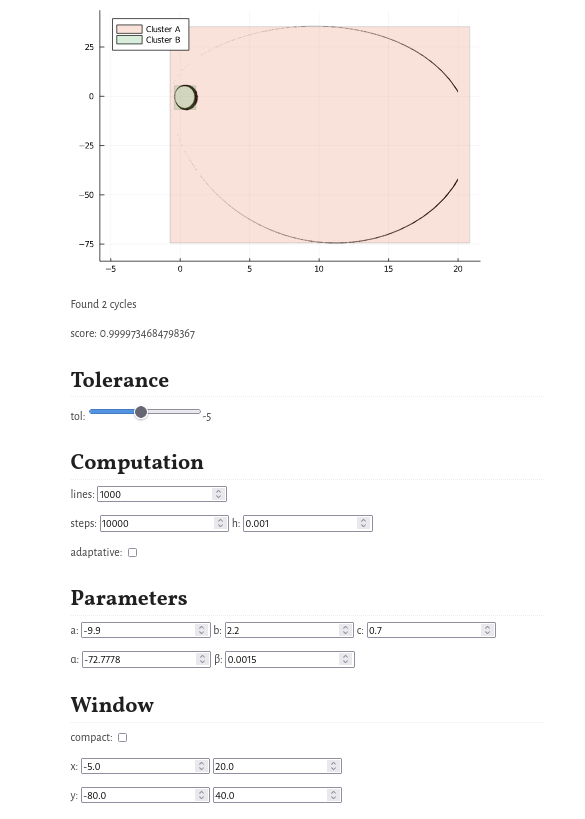
\includegraphics[width=0.4\textwidth]{pluto}
    \caption{Example of interactive Pluto notebook showing 2 limit cycles}%
    \label{fig:pluto}
\end{figure}

\subsection{OpenGL}

Another useful feature is the interoperability between \emph{CUDA} and
\emph{OpenGL}, allowing to bind the actual data used in \emph{CUDA} in the GPU
to \emph{OpenGL} textures which can be rendered directly to the screen
\cite{noauthor_opengl_nodate}. Using little modification to the program
an interactive render of the GPU data can be done.

\begin{figure}[H]
    \centering
    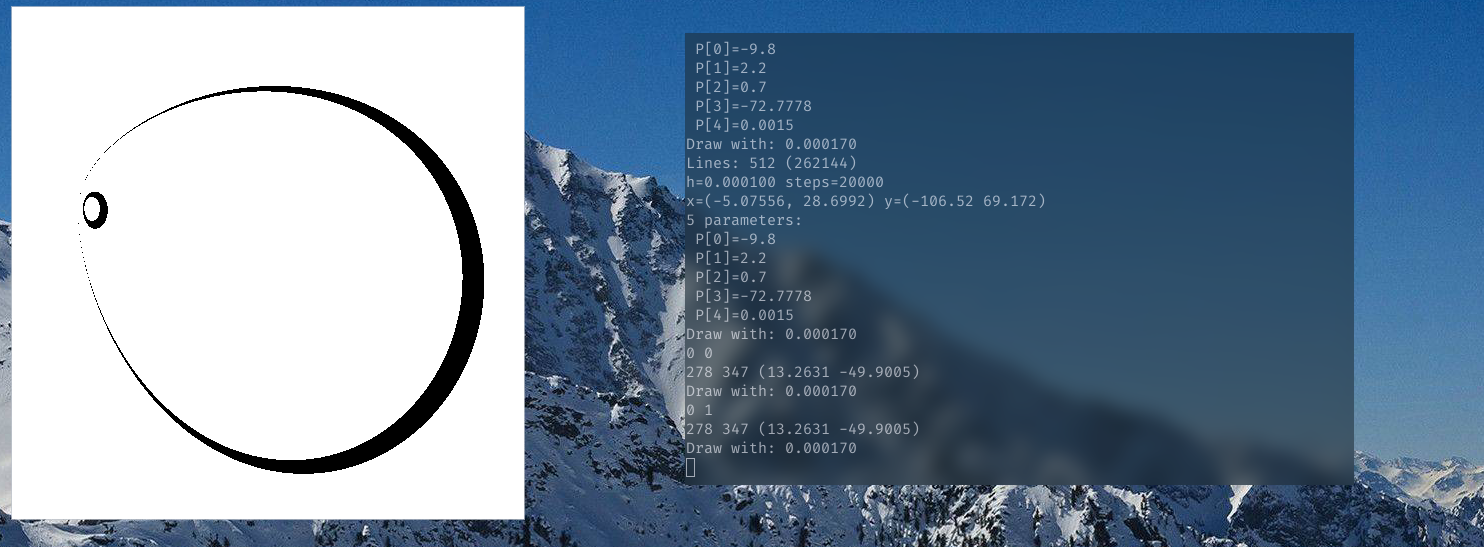
\includegraphics[width=0.8\textwidth]{opengl}
    \caption{OpenGL window directly displaying CUDA results}%
    \label{fig:opengl}
\end{figure}

\subsection{CUDA limitations on interactivity}

One of the main problems with the current implementation is that changing the system
involves creating a new \emph{CUDA} function and recompiling the library, this makes
using the program as a library quite challenging since the use must know how to
program the function and compile it. Without using \emph{CUDA} we could simply
use function pointers so that any arbitrary function can be passed and no need
for recompilation is needed. However, function pointers are extremely slow in \emph{CUDA}
since the function cannot be \emph{inlined} and we introduce massive overhead by
adding function calls to the stack.

One option is to implement a program to parse ODE systems with a strict syntax,
produces the \emph{CUDA} kernel compiles it and dynamically links it to the
program. It should be possible to do from \emph{Julia}.

    %! TEX root = **/010-main.tex
% vim: spell spelllang=en:

\section{Parameter search}%
\label{sec:parameter-search}

A parameter search was performed on the system, to obtain a table that related
the different parameter combinations with the number of limit cycles found.
Given that there where cases where a limit was not detected, the hope was

There where 5 parameters so the search space is quite large even if we only
consider a few possible values. Determining the number of cycles of a system
took~$\approx 1.5$ seconds using a $2048 \times 2048$ grid (depending on the
characteristics of the system).

\subsection{Compactified}

Since there was not enough time to compute a wide search we only applied
variations from the original parameters in \cref{eq:kuznetsov} one at a time.
2500 different values where tried for each parameter (keeping the others as
normal). This gives a total of $2500*5$ different systems to try which at
$1.5$ seconds took around 5 hours and a half. We used tangent compactification
a step size of $1^{-3}$, 20000 steps, tolerance $10^{-6}$ and \emph{Runge Kutta}
of order 3.

\subsection{Not compactified}

We also performed a smaller parameter search without applying compactification
using a window of $x, y \in (-50, 50)$ with the same search configuration.

\pagebreak
\subsection{Results}

\Cref{tab:par} shows the parameter search results for the two searches performed.
Unfortunately non of the searches found 4 or more cycles, which is to be expected since
we only varied one parameter at a time so the system was always quite close to the
original. However it shows that the compactification does obtain more results than
using an arbitrary window.

\begin{table}[H]
    \centering
    \caption{Parameter search results}%
    \label{tab:par}
    \begin{tabular}{ccccc}
        \toprule
        & 2 cycles & 3 cycles & $\geq4$ cycles & Total analyzed\\
        \midrule
        Compactified & 648 & 172 & 0 & 12500 \\
        (-50, 50) & 158 & 119 & 0 & 12500 \\
        \bottomrule
    \end{tabular}
\end{table}

Despite not finding 4 or more limit cycles some of the results where sampled from the
ones obtained to check if indeed they contained the limit cycles specified. In most cases
the number was correct. There were a few exceptions caused by applying the \emph{Kmeans}
on too little points. However these can easily be filtered out by comparing the differences
between the sizes of the cycles found.

\Cref{fig:bounding_c72} shows one of the results that gave limit cycles with
close proportions. This was found in the parameter search using the compactified
plane. In this system all the cycles are closer in size. Note that the changes in the
parameter are minimal.

\begin{figure}[H]
    \centering
    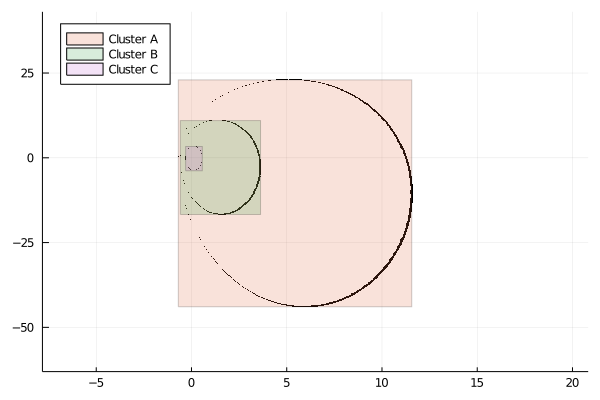
\includegraphics[width=0.8\textwidth]{bounding_c72}
    \caption{Limit cycles found on system from \cref{eq:kuznetsov} \\
        With modified parameter $c=-72.05$
    }%
    \label{fig:bounding_c72}
\end{figure}

In the search all the systems of 3 cycles found where with
very similar values to the ones in \cref{eq:kuznetsov}. The systems with 2 cycles where
much more diverse. In \cref{fig:bounding_left} there is one system in which with
$a=-27.7$ there are 2 limit cycles found, one very small around
the origin is and a much bigger one to the left. This left limit cycle is the
one which with higher parameters of $a$ we cannot detect because it increases
exponentially and the trajectories become unstable. However finding this left cycle
shows that with a capable integrator which can handle stiff trajectories the cycle should
be found in other systems.

\begin{figure}[H]
    \centering
    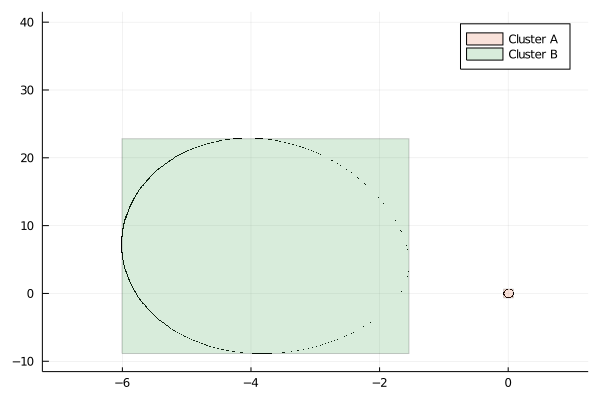
\includegraphics[width=0.8\textwidth]{left_cycle}
    \caption{Limit cycles found on system from \cref{eq:kuznetsov} \\
        With modified parameter $a=-27.7$
    }%
    \label{fig:bounding_left}
\end{figure}


    %! TEX root = **/010-main.tex
% vim: spell spelllang=en:

\section{Conclusions}%
\label{sec:conclusions}

With this project we were able to obtain a method to assist in the detection of
limit cycles by leveraging the computational power of modern GPUs. Although it is
written in \emph{C}, it integrated with other programing languages such as
\emph{Python} or \emph{Julia} allowing to visualize and further process the data
obtained.

    %! TEX root = **/010-main.tex
% vim: spell spelllang=en:
%
\section{Further work}%
\label{sec:future}

Despite obtaining promising results, many improvements can be made. Specially
regarding possible analytical methods that can help narrowing down locations of
possible limit cycles. Another area of the project that could be improved is the
integrator methods for stiff equations.
There are hundreds of well researched integration methods that far outperform the
simple \emph{Runge Kutta} methods used in the project.
Porting the implicit integrators from GNU Scientific Library to \emph{CUDA}
as some researchers have done with other parts of the library \cite{rodrigo_gnu_2019}
could enable much better integration for stiff systems.


The \emph{UAB} (Universitat Autonoma de Barcelona) has an open source program
named \emph{P4} \cite{saleta_oscarsaletap4_2018,saleta_computer_2018} to analyze
ODE systems numerically and analytically. It has the ability to find limit
cycles by computing trajectories between two points given by the user until it
reaches a cycle. This method is quite slow, in fact
in ref.~\cite{dumortier_examples_2006} there is a explicit mention on how you should
specify points very close by and reduce the precision of the computation since
otherwise the limit cycle detection may take a lot of time. The following quote
from page 267 illustrates the issue:

\begin{quote}
    A \emph{Searching for limit cycles} window  appears  with  a  time  bar
    which  should show the time left for computing but whose most useful
    application is to stop searching, since it may easily delay a lot before or
    after finding a limit cycle.
\end{quote}

Maybe our approach could be added as an alternative to assist in finding limit cycles.
Combining our program with the various analytical techniques of \emph{P4} may open new
possibilities for GPU computation of other constructs a part from limit cycles.


    %! TEX root = **/010-main.tex
% vim: spell spelllang=en:

\section{Final sustainability report}
\label{sec:sustainability-final}

\subsection{Environmental Impact}

\paragraph{PPP (project put into production)}

The environmental impact can be quantified in the number of hours of usage of
the server used to run the program.  According to the server logs, there have
been around 170 hours of server usage from the account I used. It is difficult
to estimate accurately how this translates to energy usage, but most of the time
was spent developing the program and running tests on a single system. The two
parameter searches performed where also quite small and ran for around 5 and 12
hours each using around 200 Watts on the GPU. All these estimates do not take
into account the computing time spent on my own machine or the multi-GPU
execution on the \emph{boada} server, but overall the environmental impact was
quite small.

If I were to carry the project out again, I would probably be able to use less computing
resources in the initial stages of the development of the program. During the first
iterations of the development cycle, I ran various tests that didn't really work and
took quite some time to compute.

\paragraph{Exploitation}

The main resources needed to use the project are the GPUs needed. As of now, there are
two possible use cases for the program: helping find limit cycles of a unique
system, or performing a parameter search
to find systems with interesting configurations of limit cycles.
The former can done with a simple \emph{CUDA} capable GPU and requires \emph{minimal}
resources. The latter is much more costly depending on the number of parameters to search,
it could require a powerful GPU or even a bunch of GPUs.

The program makes good use of the GPU resources, as such, it should be more energy
efficient than running the same method on a CPU or the method of computing a single trajectory
from a point until convergence used to find limit cycles with a CPU.

\paragraph{Risks}

The program is unable to find limit cycles in some cases, so it may have to be improved
in the future. If the proposed
new integrators to be able to find those cycles are implemented, there could
be a change in the resources needed to run the program. Nonetheless, it will probably
have minimal impact, since now there is still a need to run inefficient CPU code
to search stiff areas of a system.

\subsection{Economic Impact}

\paragraph{PPP}

Overall, the initial budget outlined in \cref{sec:budget} was a good estimation of the
cost of the project, there were no major problems that required modifications to the
budget nor was there any need for the contingency budget.

\paragraph{Exploitation}

As we pointed out in the \emph{PPP} section, the main cost of the project is the
computational resources to run it (what GPUs and how many are needed) as well as their
power consumption.

Right now the project needs some polishing to reach its full potential, therefore an
update may be needed in the future, probably to address the improvements
discussed in \cref{sec:future}. This will require human resources to work on the program
and maintain it.

\paragraph{Risks}

Currently, the program has been tested with a very few systems. A rigorous test on the
numerical stability of the integrators used was performed, but that is not enough to
guarantee there may not be issues with some systems.


\subsection{Social Impact}

\paragraph{PPP}

Undertaking this project I have learned a lot about general purpose graphics
processing unit programming (GPGPU) and scientific computing.

\paragraph{Exploitation}

As we mentioned on \cref{sec:future} there are researchers using similar tools
to explore constructs on ODEs and quick identification of limit cycles could
help speedup their research.

The program developed in the project does identify limit cycles quickly, but has trouble
when dealing with some trajectories. It can assist on finding limit cycles, but it is not
a complete replacement to other methods. Some parameter searches were performed but all of
them only managed to find 3 limit cycles.

\paragraph{Risks}

This project uses the proprietary \emph{CUDA} platform. Therefore, it can only be executed
on \emph{Nvidia} GPU. This makes the users dependent on this vendor since they cannot
run the program on other GPUs.




%%%%%%%%%%%%%%%%%%%%%%%%%%%%%%%%%%%%%%%%%%%%%%%%%%%%%%%%%%%%%%%%%%%%%%%%%%%%%%%%
% BIBLIO
%%%%%%%%%%%%%%%%%%%%%%%%%%%%%%%%%%%%%%%%%%%%%%%%%%%%%%%%%%%%%%%%%%%%%%%%%%%%%%%%

    \printbibliography[heading=bibintoc]

%%%%%%%%%%%%%%%%%%%%%%%%%%%%%%%%%%%%%%%%%%%%%%%%%%%%%%%%%%%%%%%%%%%%%%%%%%%%%%%%
% APPENDIX
%%%%%%%%%%%%%%%%%%%%%%%%%%%%%%%%%%%%%%%%%%%%%%%%%%%%%%%%%%%%%%%%%%%%%%%%%%%%%%%%

    % uncomment to add appendix section prefix to numbering
    \appendixpagenumbering

    \appendix

    %! TEX root = **/010-main.tex
% vim: spell spelllang=en:

\section{Appendix}


\begin{listing}[H]
    \caption{GPU hardware details}%
    \label{lst:gpu_info}
 \begin{minted}{markdown}
 Device 0: "TITAN V"
   Major revision number:                         7
   Minor revision number:                         0
   Total amount of global memory:                 12652838912 bytes
   Number of multiprocessors:                     80
   CUDA Cores/MP:                                 128
   Total CUDA Cores                               10240
   Total amount of constant memory:               65536 bytes
   Total amount of shared memory per block:       49152 bytes
   Total number of registers available per block: 65536
   Warp size:                                     32
   Maximum number of threads per block:           1024
   Maximum sizes of each dimension of a block:    1024 x 1024 x 64
   Maximum sizes of each dimension of a grid:     2147483647 x 65535 x 65535
   Maximum memory pitch:                          2147483647 bytes
   Texture alignment:                             512 bytes
   Clock rate:                                    1.46 GHz
   Memory Clock rate:                             0.85 GHz
   Memory Bus Width:                              3072 bits
   Number of asynchronous engines:                7
   It can execute multiple kernels concurrently:  Yes
   Concurrent copy and execution:                 Yes
 \end{minted}
\end{listing}


\end{document}
